\documentclass{layout/unsam-incalin-phd_v2}

\usepackage{import}
\usepackage{layout/header}

% to compile only one chapter (otherwise just comment the next line):
%\includeonly{mainmatter/theory}


%% Additional packages and commands
\setlist{itemsep=-2pt} % Reducing white space in lists slightly



%%%%% Begin of document %%%%%%%%%%%%%%%%%%%%%%%%%%%%%%%%%%
\begin{document}

%% Roman page numbering
\frontmatter

%% Defining the main parameters
\title{\thesisTitle}
%\subtitle{A Catchy Optional Subtitle \\ that Grabs the Attention}
\author{\thesisAuthor}
\affiliation{%
    \thesisAuthorAffiliation
    }

\coverimage{figures/cover.png} % Aspect ratio of 2:3 (portrait) recommended
%\definecolor{title}{HTML}{4884d6} % old color for title
\definecolor{title}{HTML}{f5ce42} % Color for title

\makecover

%%%% frontmatter
\begin{titlepage}

\begin{center}

%% Print the title
{\makeatletter
\largetitlestyle\fontsize{45}{45}\selectfont\@title
\makeatother}

%% Print the subtitle
{\makeatletter
\ifdefvoid{\@subtitle}{}{\bigskip\fontsize{20}{20}\selectfont\@subtitle}
\makeatother}

\bigskip
\bigskip

by

\bigskip
\bigskip

%% Print the name of the author
{\makeatletter
\largetitlestyle\fontsize{25}{25}\selectfont\@author
\makeatother}

\bigskip
\bigskip

%% Print table with names and student numbers
\setlength\extrarowheight{2pt}
\begin{tabular}{lc}
    Student Name & Student Number \\\midrule
    First Surname & 1234567 \\
\end{tabular}

\vfill

%% Print some more information at the bottom
\begin{tabular}{ll}
    Director: & Dra. Alejandra Tonina \\
    Co-director: & Dra. Liliana Arrachea \\
    Defense date: & Month, Year \\
\end{tabular}

\bigskip
\bigskip

%% Add a source and description for the cover and optional attribution for the template
\begin{tabular}{p{15mm}p{10cm}}
    Cover: & Corbino device, crystal grown at ETH, microprocessed at INTI by the author. \\
    % Feel free to remove the following attribution, it is not required - still appreciated :-)
    Style: & ICALIN-UNSAM report style, modified from Delft report class by Mariano A. Real (2022)
\end{tabular}

\end{center}

%% Insert the TU Delft logo at the bottom of the page
\begin{tikzpicture}[remember picture, overlay]
    \node[above=10mm] at (current page.south) {%
        
\includegraphics[width=10cm]{layout/logo/unilogo.png}
    };
\end{tikzpicture}

\end{titlepage}

\chapter*{Preface}
\addcontentsline{toc}{chapter}{Preface}

\epigraph{The story so far: In the beginning the Universe was created. This has made a lot of people very angry and been widely regarded as a bad move.}{Douglas Adams}
\epigraph{And perhaps we should avoid writing this thesis and just state that the answer to everything is 42.}{MAR}



\emph{ \\ A Caro y Uli \\ A mis viejos \\ A mi familia \\A mis directoras y colegas \\ A la nación Argentina, que con esfuerzo\\ apoya los estudios y la ciencia pública}

\begin{flushright}
{\makeatletter\itshape
    \@author \\
    Buenos Aires, \monthname{} \the\year{}
\makeatother}
\end{flushright}

\chapter*{Summary}
\addcontentsline{toc}{chapter}{Summary}

\emph{A summary...}

\chapter*{Acknowledgments - Agradecimientos}
\addcontentsline{toc}{chapter}{Acknowledgments - Agradecimientos}


% Let me thank many many people that was key to my formation and the development of this thesis. Many of them do not read English so you will find a Spanish section too.


\tableofcontents
%\listoffigures
%\listoftables
\chapter*{Nomenclature}
\addcontentsline{toc}{chapter}{Nomenclature}

\section*{Abbreviations}

\begin{longtable}{p{2.5cm}p{8cm}}
    \toprule
    Abbreviation & Definition \\
    \midrule\endhead % Abbreviations added alphabetically here:
    2DES    & 2 dimensional electron system \\
    ff      &    filling factor or filling fraction \\
    LIA     &   lock-in amplifier \\
    LL      &   Landau levels \\
    SI      &   International System of Units\\
    QPC     &   Quantum point contact \\
    ... \\
    \bottomrule
\end{longtable}

\section*{Symbols}

\begin{longtable}{p{2.5cm}p{8cm}p{2.5cm}}
    \toprule
    Symbol & Definition & Unit \\
    \midrule\endhead % Latin symbols added alphabetically here:
    $G$ & Conductance & S \\
    ... \\
    \midrule % Greek symbols added alphabetically here:
    $\rho$ & Density & [kg/m$^3$] \\
    ... \\
    \bottomrule
\end{longtable}



% Arabic page numbering
\mainmatter


%%%% chapters (mainmatter)

% You can use \input or \include. 
% \input will include the .tex right into the file like it was text in that position, i.e. you can even use it in the preface.
% \include will add a page break before and after the .tex. Also, will let you use \icludeonly{file} (see https://latexref.xyz/_005cinclude-_0026-_005cincludeonly.html) in the preamble, that becomes useful when writing your thesis to only compile a particular chapter. But you can not use it in the preface. 
% For extra info see: https://tex.stackexchange.com/questions/246/when-should-i-use-input-vs-include

\chapter[ch:foreword]{Foreword}

\textcolor{red}{meter la idea de previa que dejé en OneNote}


\chapter*{Introduction}
\addcontentsline{toc}{chapter}{Introduction}
\markboth{Introduction}{}


% The history of topological materials is just a little over thirty years old.
% A good point to start is the discovery of the quantized Hall conductance in two-dimensional semiconductor samples by von Klitzing in the early 1980s~\cite{Klitzing1980,Klitzing1992}.
% He found that the Hall conductance develops plateaus as a function of the magnetic field which are exactly quantized in multiples of a fundamental constant that depends on the elementary charge and Planck's constant.
% In particular, it is independent of any material properties or external conditions.
% Due to the high precision of the quantization levels, for which an explanation was given in the following years by Laughlin and Halperin~\cite{Laughlin1981,Halperin1982}, this effect immediately found applications in metrology as a direct measurement of the fine structure constant and as a standard for the unit of resistance.
% The discovery by von Klitzing was awarded with the 1985 Nobel Prize in physics.

% A few years after the discovery, Thouless and others discovered the first connection to topological properties~\cite{Thouless1982,Niu1985,Kohmoto1985,Avron1985,Kohmoto1989,Bellissard1994,Avron2003}.
% They found a direct relation between the Hall conductance and a topological invariant called Chern number.
% In much the same way that the number of `handles' of a closed two-dimensional manifold can be calculated by an integration over its curvature, the Chern number of a Hamiltonian can be calculated by integrating its Berry curvature over a periodic two-dimensional configuration space.
% Similar to the Gaussian curvature of the manifold, the Berry curvature of the quantum mechanical system quantifies the geometric changes of the wave functions under transport around closed loops~\cite{Berry1984,Zak1989}.
% The connection of the quantized Hall conductance to a topological invariant manifests itself in the robustness of the physical effect against local perturbations.

% A related, but considerably more complex phenomenon was experimentally discovered by Tsui, Störmer and Gossard in 1982 at even lower temperatures in cleaner samples~\cite{Tsui1982}.
% They found that the Hall conductance could additionally develop plateaus at certain fractional values of the filling factor, the ratio between the number of electrons and the number of magnetic flux quanta threading through the sample.
% These plateaus correspond to fractionally filled Landau levels and could not be explained by a single-particle treatment.
% Once again, it was Laughlin who was able to explain the phenomenon~\cite{Laughlin1983}, winning him the 1998 Nobel Prize in physics together with Tsui and Störmer.
% He found that the two-dimensional electron gas condenses into a new state of matter, a quantum fluid with fractionally charged excitations and anyonic statistics.
% This strongly correlated state of matter is an example of a topologically ordered state with a ground state degeneracy that depends on the topology of the underlying space and a robustness against local perturbations~\cite{Wen1990,Wen1995}.
% The structure of some fractional quantum Hall states still remains unexplained.
% The most prominent example is the even-denominator state at a filling of $\sfrac{5}{2}$ that was experimentally observed as early as 1987 by Willet \etal~\cite{Willett1987}.
% Particular interest in this state draws from work by Moore and Read~\cite{Moore1991}, suggesting that it might give rise to quasiparticles with non-Abelian statistics.
% Interchange of non-Abelian anyons leads to a change in the ground state manifold of the system. This property can be utilized for fault-tolerant quantum computation, an idea that has been proposed by Kitaev in 1997~\cite{Kitaev2003}

% Fundamental questions about the nature of these states as well as their prospective use in topological quantum computation spur the research in this field today.
% Traditional experiments with semiconductor samples remain challenging due to immense requirements on the sample quality, low temperatures and high magnetic fields.
% With the turn of the century and the advent of ultracold gases experiments, new ideas how to reach the Quantum Hall regime emerged.
% Unmatched control over system parameters as well as the ability to manipulate and observe on the single-particle level turn these systems into an optimal platform to advance our understanding in the field of Quantum Hall physics.
% A fundamental problem appears when trying to emulate the effect of the magnetic field.
% Electrically neutral atoms clearly do not couple to the magnetic vector potential in the way that electrons do.
% Various solutions to this problem have been proposed and experimentally implemented.
% Following an analogy that goes back to ideas by Larmor around 1900, it is possible to use a rapid rotation to induce an effective magnetic field for the neutral particles~\cite{Larmor1900}.
% In the two-dimensional system, the frequency of rotation corresponds to the effective magnetic field strength parametrized by the cyclotron frequency.
% Likewise, the Coriolis force is in one-to-one correspondence with the Lorentz force.
% Starting in the early 2000s, experiments in this respect have advanced over the years~\cite{Schweikhard2004,Bretin2004,Cooper2008,Fetter2009}.

% An alternative route was followed by Haldane~\cite{Haldane1988}.
% In 1988, he proposed a lattice model with broken time-reversal symmetry which showed a quantum Hall effect without the requirement of Landau levels that would be generated by an external magnetic field.
% The Haldane model utilizes complex tunneling phases that respect the symmetry of the lattice and generate a topological band structure.
% It is a showcase for a class of materials called Chern insulators.
% They behave similar to ordinary band insulators, but have conducting states at the edge of the material: a physical manifestation of their non-trivial Chern number~\cite{Hatsugai1993}.
% For charged particles, the required complex tunneling phases are connected to the external magnetic field through a Peierls substitution~\cite{Peierls1933}.
% In this regard, synthetic magnetic fields can be created for neutral particles by realizing complex tunneling phases.
% Powerful approaches are optical flux lattices~\cite{Cooper2011}, laser-assisted tunneling~\cite{Aidelsburger2011,Aidelsburger2013,Miyake2013,Kennedy2015} or lattice shaking methods~\cite{Struck2012,Struck2013}.
% The latter has recently been used by Jotzu \etal to realize the Haldane `toy model' with ultracold fermions in an optical lattice~\cite{Jotzu2014}.

% Finally, another strategy is to use spin-orbit coupling techniques~\cite{Lin2011,Cheuk2012,Wang2012,Hamner2014,Jimenez-Garcia2015} to realize topological phases.
% The interplay between external and internal degrees of freedom can lead to phenomena which are similar to the magnetic field counterparts.
% In 2005, Kane and Mele showed that spin-orbit coupled electrons in graphene can realize a topological system which encapsulates two time-reversed copies of Haldane's model~\cite{Kane2005a,Kane2005}.
% The resulting arrangement is an example for a time-reversal invariant topological insulator. It shows a quantum spin Hall effect where the two spin-components have a Hall conductance with opposite sign~\cite{Qi2011,Hasan2010}.
% A physical realization in semiconductor quantum wells was proposed by Bernevig \etal in 2006~\cite{Bernevig2006a,Bernevig2006b} and experimentally demonstrated by König \etal one year later~\cite{Konig2007}.

% A variety of experimental methods to probe topological materials have been established in recent years.
% Edge states have been observed in different systems like silicon photonics~\cite{Hafezi2011a,Hafezi2013}, photonic lattices~\cite{Rechtsman2013} and phononic mechanical systems~\cite{Susstrunk2015}.
% Furthermore, the perfect control over ultracold atomic systems has led to new ways to directly measure topological properties like the Zak phase~\cite{Atala2013}, the Berry curvature~\cite{Duca2014} or the Chern number~\cite{Aidelsburger2014}.

\textcolor{red}{Include a thermopower review, i.e. small recount of thermal responses measurements in Corbino and Hall bars. Cite here works and make sure to include Molenkamp, Benenti, Koba, Zalinge papers. }

The quantum Hall effect (QHE) \cite{klitzing1980new} is one of the cornerstones to electrical metrology and the redefinition of units of 2019 \cite{CGPM26}. It was already in the hart of the adendum of the 1990 revision of the SI, then, the electrical metrology comunity was alowed to use quantum standards kind of outside the SI. Its link being the calculable capacitor. There are many advisable works regarding this point like \cite{Valdes2019}
, and a versatile playground for solid state physics since its discovery more than 40 years ago \cite{klitzing1980new}.

As mentioned before this thesis original focus was on the study, development and implementation of methods to determine the temperature of systems under the quantum Hall (QH) state. Furthermore, it also covered possible new thermal effects under this fascinating system. Regarding the latter, we were able to grasp a promissing cooling behavior, that will be presented in \textcolor{tmagenta}{citar acá el capítulo de cooling}.

Studying the thermopower effects under the QH regime is a particular difficult task, and caught the attention of many works in the past \cite{chickering2010,chickering2010thermopower,chickering2013,kobayakawa2013diffusion} \textcolor{tmagenta}{citar los trabajos que midieron themopower antes}. But the results usually presented some issues regarding consistency and interpretation, this was pointed out by Y. Barlas and K. Yang \cite{Barlas2012}. They showed that the use of devices with a Hall-bar geometry presented intrinsic problems because of the voltage component mixing, resulting in a misalignment between the voltage and temperature gradients in the devices. They also presented an elegant solution, by proposing a Corbino (ring shaped) geometry, that imposes the gradients to be parallel. When working on this problem their focus was on the study of new possible non-abelian physics in the $ 5/2 $ fractional state. This was experimentally studied, in Hall-bar geometry, by the 
Eisenstein group \cite{chickering2010,chickering2013}, the Molenkamp group \textcolor{tmagenta}{citar molenkamp y otros trabajos en esta dirección}. But our focus is in a different direction, we exploited this work to produce new methods and approach to determine temperature gradients, thermal properties and possible new applicable effects of the QH states. 



 Two very interesting side of the effects are its thermal and thermoelectric properties, for which many insightful works have been produced \cite{chickering2010thermopower,chickering2013thermoelectric,VanHouten1992,Zalinge2003,endo2019spatial,Liu2018} \textcolor{red}{citar trabajos de chickering, molenkamp, von klitzing etc sobre estos estudios}. 

In this kind of studies to measure the 2D electron system (2DES) temperature or temperature gradient is of main importance. But many times one relies on a typical resistance transducer, that, depending on the kind of measurement, might be not the best suited configuration for the measurement in hand.


Thermoelectric voltages are a consequence of a temperature gradient along the electronic system. 
In a traditional experiment the usual configuration is a hall bar \cite{chickering2010thermopower,chickering2013thermoelectric} \textcolor{red}{citar aquellos con hall bar}, where one end of a rectangular sample is clamped to a thermal bath while the temperature at the other is increased by means of some kind of heating system, leading to a temperature distribution along the length of the sample. This configuration presents some issues, because it mixes longitudinal and transverse responses as described by Barlas and Young in \cite{barlas2012thermopower}. They show that a Corbino device averts the problem, for which its geometry imposes a parallel thermal gradient to the electrical potential drop (thermopower). Some works have taken advantage of this geometry and its possibilities \cite{Zalinge2003,kobayakawa2013diffusion,real2020thermoelectricity,mateos2021thermoelectric}. 
However, a thermal gradient cannot be straightforward applied in a ring-shaped Corbino structure where the center of the ring should be heated and the rim be cooled. 
It turns out to be difficult to connect the outer rim of the Corbino to a thermal bath with a vanishing thermal resistance. 
Another issue being the high thermal conductivity of the substrate which leads to small thermal gradients at reasonable heater powers. \textcolor{blue}{In a different approach van Zalinge et al. \cite{Zalinge2003} used illuminated samples, a laser acting as a hotspot probe and using it to study anisotropies in the photo and thermovoltages. They found anisotropies regarding the thermovoltage responese to the different main directions of the crystal.} Kobayakawa et. al\cite{kobayakawa2013diffusion} used a Corbino configuration having its center connected to a thermal sink while a circular rf heater surrounded the ring, and focus in low mobility and low magnetic fields. 

In this work we use a more conventional approach, which consists in placing  a central resistive heater and gluing a rim of the sample to the chip carrier, thermally connected to the cold finger of a $^3$He cryostat. Taking advantage of the temperature dependence of the conductance minima in the quantum Hall (QH) regime we experimentally estimate the thermal gradient produced along the sample for different heater powers and base cryostat temperatures. We demonstrate that there exists a linear relation between the power applied to the heater and the temperature gradient in the sample. The good agreement found suggests a potential application of the device for sensing small temperature biases in micro and nano devices. The Corbino device we study is schematically showed in Fig.~\ref{fig:fig1-expSetup}.
\chapter{Theoretical introduction}
\label{ch:theory}

\section{Thermoelectricity in the quantum realm}
\label{sec:teo:teoThermoQH}

A central concept we will exploit is the use of a \textit{transmission function} $\mathcal{T}$ as means to model different aspects of our coherent systems. Since we are dealing with non-equilibrium thermodynamics we will be using known results of linear response theory and Onsager reciprocity relations \cite{onsager1931reciprocalI,onsager1931reciprocalII}, extended later by Mazur and de Groot \cite{mazur1953onsager} to systems under external magnetic fields. 
We will follow many times a beatifull and extended review by Benenti, Casati, Saito and Whitney \cite{benenti2017fundamental} on this subject matter, in many cases we will not go deep into the theory, in those cases this review already covers it perfectly. A second review of main importance is the one by Giazotto, et. al. \cite{Giazotto2006Mar}, where the theoretical approach is deeply embedded of experimental examples, and is also an important source of information on the subject.

One could argue about the time-reversal symmetry and its consecuences, but it has been taken into consideration recently \cite{luo2020onsager}.

A key argument is that we will be dealing always with low dimensional systems that can be modeled as two terminal systems, having chiral (directional) coherent channels connecting these terminals, as shown in Fig.~\ref{fig:teo:2terminal}. 

As we have briefly mentioned, topologycal insulators (as the quantum Hall state) provide such particular configurations. Lets discuss then the basic mathematical approach that we will use latter.

\begin{figure}
    \centering
    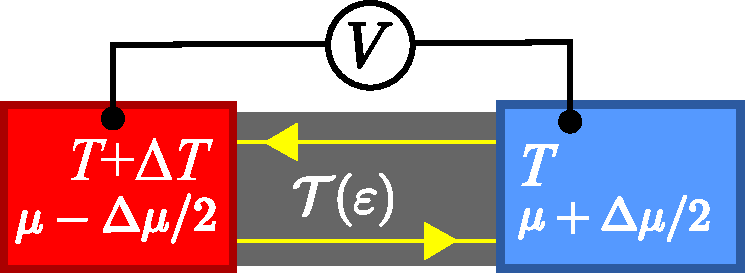
\includegraphics[width = 0.5\textwidth]{figures/theory/2-terminal.pdf}
    \caption{Schematic view of a typical topological system having two coherent chirial edge channels. It is also included a possible difference in temperature and chemical potential between contacts. Such systems can be completely described by a transmission function $\trans(\varepsilon)$. A configuration like this will produce a voltage accordingly, here indicated to be measured by the ideal voltmeter $V$.}
    \label{fig:teo:2terminal}
\end{figure}


In linear response, the corresponding charge and heat currents for small  $\Delta T$ and bias voltage $V$
 can be expressed as \cite{benenti2017fundamental}
 %
\begin{equation}
\label{eq:thermoLinearMatrix}
    \left(
        \begin{array}{c}
            I^c/e \\
            I^q 
        \end{array}
    \right)  
    =  
    \left(
        \begin{array}{cc}
            \onsa{11}   &   \onsa{12}  \\
            \onsa{21}   &   \onsa{22} 
        \end{array}
    \right) 
    \left(
        \begin{array}{c}
            e \text{V} / k T\\
            \Delta T / k T^2
        \end{array}
    \right),
\end{equation}
%
being $\hat{\cal L}$ is the Onsager matrix \cite{onsager1931reciprocal, onsager1931reciprocalII}, wile the right vector contains the so called generalized forces. Here $I^{c(q)}$ is the charge(heat) current, $e$ the quantum of electrical charge, $k$ the Boltzmann constant, V the voltage across the system and $T, \Delta T$ the temperatures. 

This leads to the definition of the usual thermoelectric variables:
\begin{itemize}
  \item The electrical conductance $G=e^2 \onsa{11}/T$
  \item The thermal conductance $\kappa= \det{\hat{\cal L}}/\left(T^2 \onsa{11} \right)$
  \item The Seebeck coefficient $S  = \onsa{12}/ \onsa{11}$
  \item The Peltier coefficient $\Pi= \onsa{21}/ \onsa{11}$
\end{itemize}

For ballistic or diffusive transport  ${\cal L}_{ij}$ depends only on the quantum dynamics of the electrons in the presence of the magnetic field and the disorder of the sample. They are  described by a transmission function $\trans (\varepsilon)$,
%
\begin{equation}
  \label{eq:teo:onsaCoef}
  \onsa{ij}= - T \int  \frac{\partial f (\varepsilon)}{\partial \varepsilon} \left(\varepsilon-\mu \right)^{i+j-2} {\cal T}(\varepsilon) \frac{d\varepsilon}{h},
\end{equation}
%
where  $f(\varepsilon)=1/(e^{(\varepsilon-\mu)/k T}+1)$ is the Fermi-Dirac distribution function, $\mu$ is the chemical potential and $T$ is the temperature of the carriers. 

We will apply this formalism to a specific initial problem in the next section, it will allow us to understand its consequences and possibilities. As we have discussed such studies in quantum coherent systems are of great significance in order to control heat to work conversion, heat distribution, carrier heat transport, heat filtering, thermovoltage, peltier effect, between many others \textcolor{red}{citar papers de control térmico de electrones en estados coherentes en cada uno de los ejemplos dados}.


\section{Topological insulators and Onsager}
\label{sec:teo:onsaTopo}


During the initial course of this thesis, when  learning the Onsager formalism, the idea to study thermoelectricity and heat control also in quantum spin Hall states (QSH) was suggested. Having the possibility to apply both, the tools in need and to explore the new realm of two-dimensional (2D) topological insulators (TIs). This systems are another beautiful realization of quantum coherent transport.\textcolor{red}{agregar citas de choerent transport}

Like the quantum hall state, the quantum spin Hall  hosts edge states (channels)\cite{nowack2013imaging}, 
examples being \ce{MnBi2Te4 / Bi2Te3} heteroestructures and \ce{CdTe/HgTe} quantum wells \cite{konig2008quantum, Koenig766,bernevig2006qsh,bernevig2006prl}. 
Unlike the QHE they do not require magnetic fields to be applied, here the particular band structure of the system produces a sequence of states resulting in the quantum spin Hall (QSH) state. It take place in 2D-TIs, and preserves time-reversal invariance. Hence, helical pairs of edge states appear, these are the \textit{helical Kramers pairs} \cite{kanemele2005,bernevig2006quantum,Koenig766, Roth2009} having opposite spin orientations determined by the spin orbit of the system.

We will not go deeper into these impressive systems, bibliography already covers them, for example \cite{maciejko2011quantum, konig2008quantum}. Also very interesting information can be found at groups webpages, particularly \url{https://www.bernevig.com/} and \url{https://imprs-cpqm.mpg.de/93235/LP_Molenkamp}.

Finally, 2D-TIs will be in the future of metrology, recent works by the Electrical quantum metrology group at PTB (Physikalisch-Technische bundesanstalt) and Molenkamp group at MPI (Max Planck Institute) have demonstrated the universality of the effect applying cutting edge metrology to \ce{V_{0.1}(Bi_{0.21} Sb_{0.79})_{1.9}Te3 } compounds \cite{gotz2018zero}. 


\subsubsection{Thermoelectric performance in the quantum coherent regime}

The initial theoretical (but realistic) problem studied, consisted in the device shown in figure \ref{fig:teo:QSHscheme}, an original idea of Dr. Arrachea that was developed with D. Gresta and myself \cite{Gresta2019}.

\begin{figure}
    \centering
    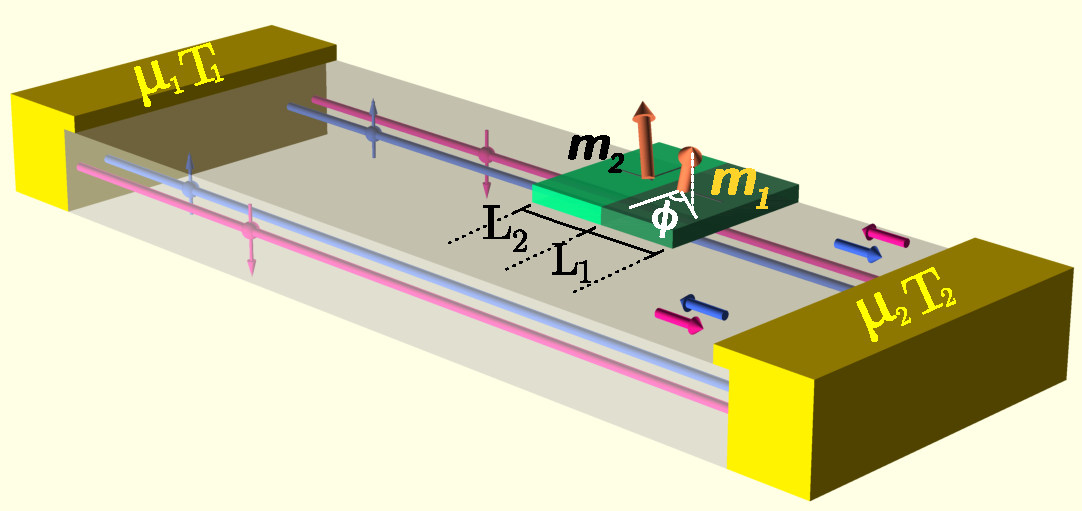
\includegraphics[width = 0.7\textwidth]{figures/theory/QSHscheme.pdf}
    \caption{Sketch of the setup scheme. 2D TI contacted to ohmic contacts at which a bias voltage $e$V$ = \mu_1−\mu_2$ and temperature difference $\Delta T = T_2 - T_1$ are applied. Two nano-magnets having moments $\textbf{m}_1$ and $\textbf{m}_2$ and lengths $L_1$ and $L_2$, are contacted to a helical Kramer's pair of edge states.}
    \label{fig:teo:QSHscheme}
\end{figure}

The system consist on a 2D topological insulator having two ohmic contacts at different temperatures ($T_1, T_2$) and chemical potentials ($\mu_1, \mu_2$), and two nanomagnetic islands over a side of the sample, only affecting one pair of the helical edge states. We shall start by studying a single island and then consider two of them, having different magnetic moments. The relevant physical property will be the the finite component of those moments perpendicular to the direction of the spin-orbit interaction of the 2D-TI, similar systems were considered in Refs. \cite{silvestrov2016noiseless,arrachea2015nanomagnet}. The system can also be studied to produce topological superconductivity \cite{Fu2009}.  

Such system is coherent, so its transport properties do not present inelastic scattering processes, and can be \textit{fully characterized by a transmission function.} Furthermore, the off-diagonal components $\mathcal{L}_{12} = \mathcal{L}_{21}$ are the ones encoding the thermoelectric heat to work conversion. 
As a general rule, when searching for optimal thermoelectric systems, one must search for systems having a rapidly changing transmission function within the relevant transport window. In those energy ranges we will be able to break the particle-hole symmetry, a necessary condition for heat to work conversion. 

This idea is key throughout this thesis, particularly when studying thermoelectricity in the quantum Hall state, in which the mentioned change is obtained on the sides of the mobility gap, see \ref{ch:vtp_g_model}.

The performance of the system is usually measured by the \textit{figure of merit ZT}, being its limit the one of Carnot, then $ZT \rightarrow{\infty}$, obtained for delta-shaped distributions \cite{mahan1996best}. Meanwhile, thermoelectric heat engines (power from heat) is optimized for the case of Heaviside step functions.

Typical temperatures for such devices mean to work at sub-kelvin temperatures to ensure full quantization, even when theoretically some of them should perform up to \SI{100}{\kelvin} \cite{pan2020probing}. Regarding the magnetic islands, let us start by considering a single magnetic domain having a magnetization $\textbf{m}$, which projection to the perpendicular direction to the helical states is $\phi$ and having a length $L$. 

\textcolor{red}{Probably I could skip the Hamiltonian, just state the mag moment and say that: Solving the Dirac hamiltonian plus the magnetic interaction, eq. \ref{eq:teo:magMoment} to the Kramer's pairs \cite{BustosMarun2013,Gresta2019,Gresta2021PhD}, we find the transmission function to be... }
To obtain the  transmission function one must start by modeling the system via the usual Dirac Hamiltonian of the Kramer's pairs plus a magnetic interaction
\begin{equation}
\label{eq:teo:hamiltonianQSH}
    \textit{H} = 
        \int{
        \Psi^\dagger(x)
        \left[ 
            \left( 
                -i\hbar \upsilon_F \partial_x
            \right) 
            \hat{\sigma}_z + J \, \textbf{m}(x) \cdot \hat{\boldsymbol{\sigma}}
        \right]
        \Psi^\dagger(x)
        }
\end{equation}
the Kramer's pairs wave-functions $ \Psi(x) = \left( \psi_{R \uparrow}(x),\psi_{L \downarrow}(x) \right)^T $ include the right (left) moving carrier channels having velocity $\upsilon_F$ and $\uparrow ( \downarrow )$ spin orientation. $J$ represents the magnetic exchange interaction between the magnetic moment of the island and the spin of the carriers. Finally, $\hat{\mbf{\sigma}} = \left( \hat{\sigma}_x,\hat{\sigma}_y, \hat{\sigma}_z \right)$ are the usual Pauli matrices.

Meanwhile, the magnetic moment is given by
\begin{align}
\begin{split}
\label{eq:teo:magMoment}
    \textbf{m}(x) &= \sum_{j=1}^N{\Theta(x_j - x)\Theta(x - x_{j-1}) \, \textbf{m}_j}\\
    \textbf{m}_j &= (m_{j\perp} \cos{\phi_j}, m_{j\perp} \sin{\phi_j}, m_{j\parallel}) 
\end{split}
\end{align}
%
$\textbf{m}_j$ being the magnetic moment per unit length of the islands having lengths $L_j = x_j - x_{j-1}$. Here $\perp$, $\parallel$ means respect to the direction of the spin orbit interaction of the TI. 
We shall start by discussing the $N = 1$ problem and mention some interesting additional effects when $N = 2$.

\subsubsection{Single domain case}
Solving this Hamiltonian problem as in Refs.~\cite{BustosMarun2013,Gresta2019,Gresta2021PhD} results, for the case of a \textit{single magnetic island} $N=1$, in the following transmission function 
\begin{align}
    \label{eq:teo:transFuncQSH}
    \trans(\varepsilon) &= \frac{\mid \varepsilon^2_\perp - \varepsilon^2 \mid}{\mid \varepsilon^2_\perp - \varepsilon^2 \mid \cos^2{\lambda} + \varepsilon^2 \sin^2{\lambda}}\\[2ex]
    \lambda &= \frac{L}{L_0}\sqrt{\left( \varepsilon/\varepsilon_{\perp} \right)^2-1} = lr 
\end{align}
where $\varepsilon_{\perp, \parallel} = J m_{\perp, \parallel}$, $l = L/L_0$, $L_0 = \hbar \upsilon_F/\varepsilon_{\perp}$ and  $r=\sqrt{\left( \varepsilon/\varepsilon_{\perp} \right)^2-1}$. It is important to note two things regarding the transmission function:
\begin{itemize}
    \item Only depends on the perpendicular projection of the moment $m_{\perp}$ to the spin-orbit interaction of the material. 
    \item It is symmetrical respect to $\varepsilon =0$, this means that there is an effective coupling of the Kramer pairs, resulting in a gap opening in $\varepsilon_{\perp}$ if the magnetic island es large enough.
\end{itemize}

The resulting behavior of the system is shown in Fig.~\ref{fig:teo:tau1isla}, where the horizontal axis is normalized to $\varepsilon_{\perp}$. As mentioned, we find a gap opening if $L > L_0$, before that, the tunneling its strong. $l$ ratios higher than 4 results in a well defined gap, and as the ratio increases oscillations become denser and narrower.
%
\begin{figure}
    \centering
    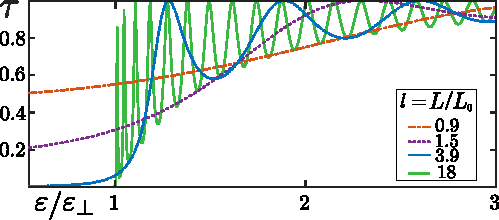
\includegraphics[width = 0.7\textwidth]{figures/theory/fig2.pdf}
    \caption{Transmission function $\trans$ of the system as a function of the energy normalized to $\varepsilon_{\perp} = J m_{\perp}$, that determines the energy of the gap for a proper magnetic island length $L$. The different curvs corresponding to changes in the ratio $l = L/L_0 = L/\hbar \upsilon_F/\varepsilon_{\perp}$, note that for ratios higher than 4 a gap is already defined, and oscillations become relevant outside the gap. Higher ratios results in denser and narrower oscillations.}
    \label{fig:teo:tau1isla}
\end{figure}
%
Note that wider islands results in a higher oscillating transmission function outside the gap. Such behavior will become highly interesting from the point of view of heat to work optimization, since a delta-like transmission functions should be ideal in this sense. But that is not the whole story, if we consider the way we must evaluate the Onsager coefficients \onsa{ij}, they depend on the temperature, and if it is high enough the integration in eq.~\ref{eq:teo:onsaCoef} will smooth such oscillations, even to the point where no effect is obtained. So, there is a very interesting interplay between the magnetic island length and the temperature gradient to use, this will become relevant again and again during the course of the thesis.









\begin{figure}
    \centering
    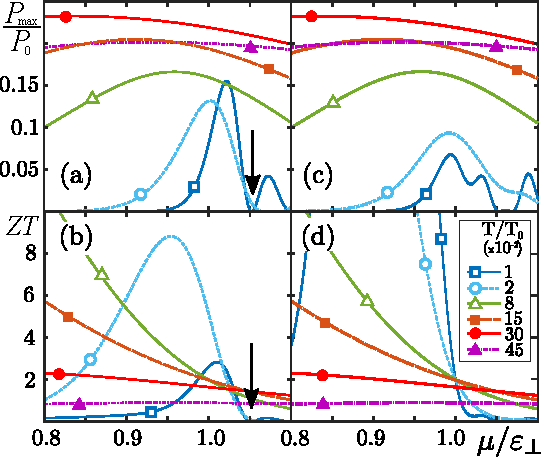
\includegraphics[width = 0.5\textwidth]{figures/theory/fig3.pdf}
    \caption{power and ZT}
    \label{fig:teo:powerZT}
\end{figure}

\begin{figure}
    \centering
    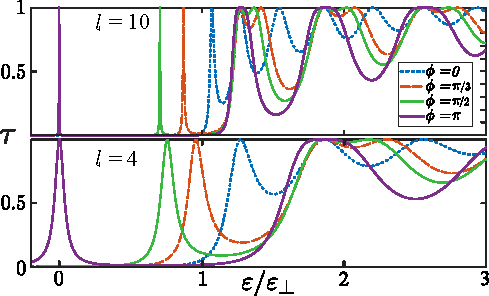
\includegraphics[width = 0.5\textwidth]{figures/theory/fig4.pdf}
    \caption{Tau for two islands and different L}
    \label{fig:teo:tauDiffL}
\end{figure}

\begin{figure}
    \centering
    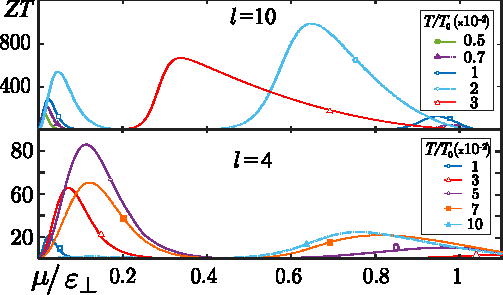
\includegraphics[width = 0.5\textwidth]{figures/theory/fig5.pdf}
    \caption{power and ZT two islands different L}
    \label{fig:teo:powerZTDiffL}
\end{figure}


\begin{figure}
    \centering
    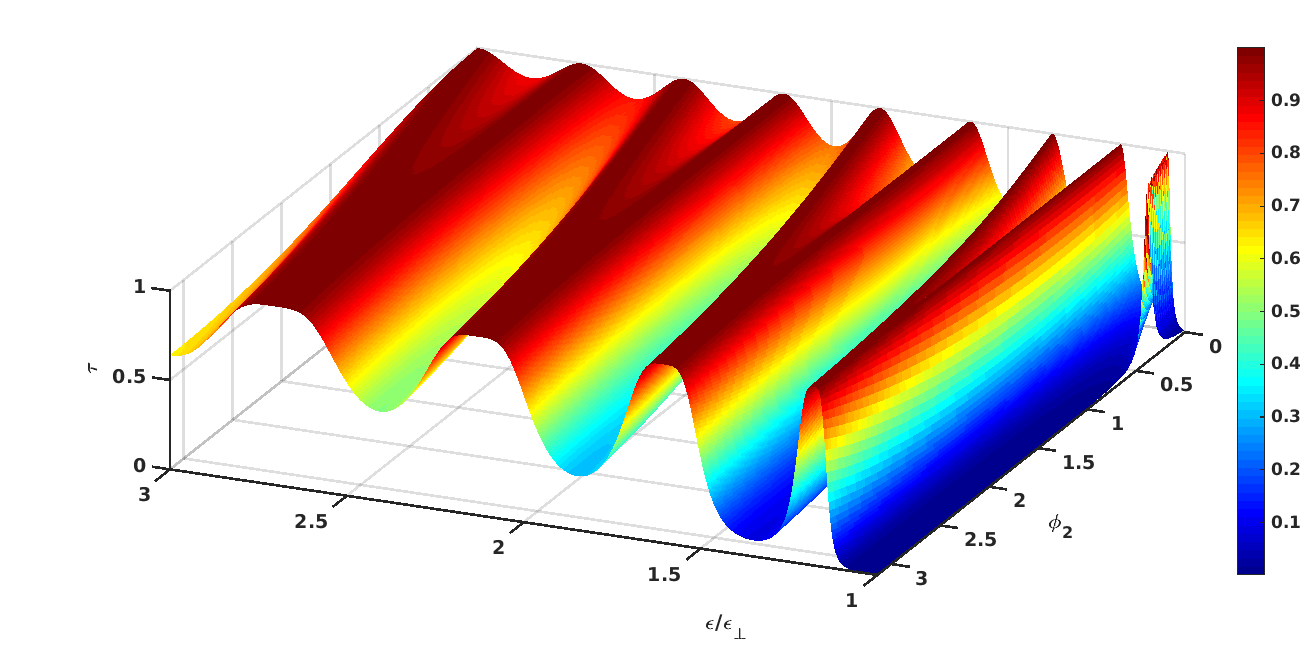
\includegraphics[width = 0.5\textwidth]{figures/theory/Tauenerphi.png}
    \caption{Tau for changing relative angle}
    \label{fig:teo:tauDiffangle}
\end{figure}
\chapter{Experimental approach}

Given the already exposed, we concentrated in Corbino ring devices, but the question remained as which heating method was to be used. The approach by Kobayakawa, \etal \cite{kobayakawa2013diffusion} is very cleaver but implies the use of high frequencies, which increases the complexity of the measuring system. Also, one could argue about how the system could follow such high frequencies, they use microwaves and a co-planar arrangement to this end. Also the themovoltage developed in the system (we will return to this concept afterwards) is measured by a central inner ohmic contact and two outer quasi-Corbino contacts, if the system has a preferred direction, are they actually measuring the proper voltage? For example in the work by van Zalinge, et. al. \cite{Zalinge2003} it is argued that the thermopower is not isotropic, again, more on this to come.

It was decided to opt for a very conservative heating system, a heating resistor to be included outside the mesa. And two approaches were considered, 1- a central heater or 2- a outer heater. The advantage on the second was that could be designed to have a much greater power, but would be hard to ensure its homogeneity, the termination would include a possible anisotropy (has to be open at the end), between some other electrical possible effects as capacitance \textcolor{tmagenta}{incluir referencia a la figura del heater por fuera (buscar el diseño que había hecho)}, inductance and such. 
So, a central heater was decided, which had to be small to resemble as much as possible a point heating system and support as much power as possible to overcome the cooling power of the cryostats to be used. For example, in the case of a wet \(^3\)He cryostat, in one hand the Helium would fight very hard against heating, but it is also possible that increasing the heating power ends in the Kapitza effect \textcolor{red}{citar acá dicho effecto} that could suddenly increase dramatically the heating power, taking the system out of regime or burning it. There, the He becomes gas, icreasing the heat capacity, increasing its temperature and resulting in an increased temperature transfer to the sample, because of both, the gas and the crystal.

\subsection{Experimental set-ups}
\label{subsec:experimental_setup}
Several measurement set-ups were tested. Usually in the laboratory we perform a regular DC measurement when working on Hall-bar samples. But in the case of thermopower it became nearly mandatory to switch to an AC approach, Fig.~\ref{fig:corbino_exp_setup}. Since we committed to a central heater and we must measure voltage and temperature responses one finds a two-fold problem: how to only measure the thermopower (thermovoltage) response \textit{only} and how to measure acurately the resulting temperature gradient produced by the heater.

\begin{figure}
    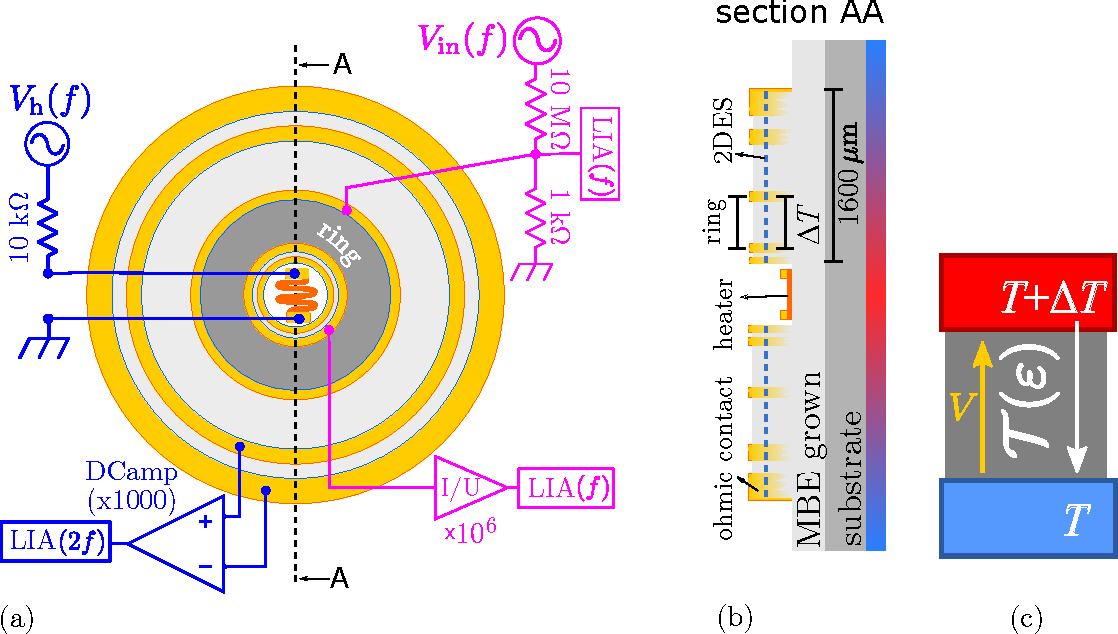
\includegraphics[width=1\textwidth]{figures/experimental/cobino_exp_arangement.pdf}
    \caption{A typical device scheme is shown. Notice the several concentric Corbino devices, they act independentrly during measurements (see text). (a) Experimental setups: \textcolor{blue}{blue} configurations are intended to measure thermopower, \textcolor{magenta}{pink} configuration is used to produce conductance measurments of the system. We will denote the innermost Corbino ring 1, then 2, and the outermost will be ring 4. (b) Section cut AA of the schematic device depicted in (a), notice that the central resistive heater is outside the mesa and will induce a radial heating on the samples. (c) Scheme of the two contact device we think of when modeling the system. Being the hot contact the inner ohmic Corbino contact, and the cold one the outer ohmic Corbino contact. \textcolor{red}{incluir luego un panel adicional con fotos de los dispositivos.}}
    \label{fig:corbino_exp_setup}
\end{figure}

The first problem has been overcome before by Molenkamp \etal \cite{molenkamp1993QPCthermal}, when studding thermoelectric responses in QPCs. They demonstrated that one can measure the thermovoltage responses by lock measuring the second harmonic response of the system to the heating device. 

So, an AC voltage $V_\text{h}$ resulting in a current $I(t)$ of frequency $f$ is applied to the heater, and it's seccond harmonic response will be measured by a lock-in amplifier (LIA)
\begin{equation}
    \label{eq:heater_current}
    I(t)=I_0\sin(\Omega t + \varphi), 
\end{equation}
with \( \Omega= 2\pi f \), and \( \varphi \) a possible arbitrary phase. This translates into the power,
\begin{equation}
    \label{eqs2}
    P(t)= \frac{R I_0^2}{2} \left[1- \cos(2 \Omega t + 2 \varphi) \right],
\end{equation}
where \(R \) is the heater resistance.

Thus, a temperature bias is generated between the heater and the external rim of the structure which has a constant component and one that oscillates with the frequency $2 f$. 
In \textcolor{red}{citar seccion dependencia potencia con temp medida}, we show that there exists a linear relation between the power and the temperature bias. Therefore, it is natural to assume the following behavior for the temperature bias,
\begin{equation}
    \label{eq:deltaT_time}
    \Delta T (t) = (\Delta T)_0 - (\Delta T)_2 \cos (2 \Omega t + 2 \varphi).
\end{equation}

At very low frequencies and under ideal conditions, $(\Delta T)_2$ should be independent of the frequency and equal to $(\Delta T)_0$. We shall come back to this point later on. 
Consequently, the developed thermovoltage has a constant component plus an oscillating component of frequency $2f$, this is 
\begin{equation}
    \label{eq:vtp_time}
    V_{tp}(t)=V_{ tp \, 0} - V_{tp \, 2} \cos (2 \Omega t + 2 \varphi).
\end{equation}

The experimental setup is designed to measure the oscillating component $ V_{tp \, 2}$ of the thermovoltage. 
The Seebeck coefficient $ S={\cal L}_{12}/{\cal L}_{11} $ relating the thermovoltage with $ \Delta T $ depends on the microscopic mechanisms behind the transport processes. 
Within linear response this quantity is expected to be the same for the constant and oscillating components of $ \Delta T $ and $V_{tp}$. 
Notice that in this type of measurement there is a $3\pi/2+\varphi$ phase lag between the oscillations of the injected current and the measured thermovoltage. 
The measurements we show in this text have a $\varphi=0$ injected signal phase and the corresponding 2nd harmonic in the signal of $ V_{tp} $ has a phase lag of $3\pi/2$ within the Landau levels, in full agreement with Eqs. (\ref{eq:heater_current}) and (\ref{eq:vtp_time}). 

However, as we will discuss in \textcolor{red}{citar seccion vtp meas} within the gaps between Landau levels the response shows spike like voltages, which have also other phase lags, and out of phase huge responses. The origin of the latter features were a striking feature and required an important amount of work to understand. We will get back to them, but let us state that for the time being we have a culitative explanation to them, and deserves future investigations.

From the technical point of view, it is important to chose the proper frequency range. We studied the thermopower response at different frequencies and found an upper limit at $f = \SI{100}{\hertz}$, i.e. $2f = \SI{200}{\hertz}$ where the voltage started to decrease with increasing frequency. On the other hand, the total cryosystem has a characteristic thermal-relaxation corresponding to a frequency below \SI{1.5}{\hertz}. These two frequencies determine the frequency range that could be used during thermopower measurements, we have use \SI{13.838}{\hertz} unless otherwise stated.

The conductance measurements were not constrained by these limits, because the additional power dissipation was always negligible. A higher frequency of \SI{113}{\hertz} increased the accuracy and reduced the measurement times, which was particularly relevant for the temperature calibration, to be discussed in section~\ref{temperature_corbino}. In the QHE regime the internal resistance of the thermal voltage can become very high. Its measurement requires a DC amplifier with very high input impedance. We use an amplifier with about \SI{10}{\tera\ohm} input impedance and differential guarded inputs \cite{Maerki2017}.

We verified that the measurement of the voltage across the radius of the device is indeed generated by a thermoelectric effect rather than being induced  by a time-dependent magnetic field. The latter effect would actually be the experimental realization of Laughlin's {\em gedanken} experiment \cite{laughlin1981quantized}. According to this, a time-dependent magnetic flux threading  the Corbino ring would induce an electrical field given the induced emf by Faraday law, causing eddy currents circulating along the circumferences of the structure, which would lead to the development of a radial Hall voltage. Such voltage would depend on the time-derivative of the magnetic field. 
Thus, the measurements have been performed by changing the magnetic field in steps using different waiting times to allow the thermovoltages and magnet to stabilize.

In addition, we made voltage measurements in the thermovoltage configuration (see Fig.~\ref{fig:corbino_exp_setup}) both within the Landau levels and within the gapped regions with the magnetic field pointing in opposite orientations.
We did not find any signature of an effect due to a time-dependent magnetic flux, as the ones discussed by Dolgolopov, \etal\cite{dolgopolov1992quantum,dolgopolov1993charge}. There they produce measurements in both magnetic field directions, and showed that in such cases we could expect a toothsaw-like response wich sign would be dependant of the magnetic field derivative, as sown in Fig.~\ref{fig:dolgo}.

\begin{figure}
    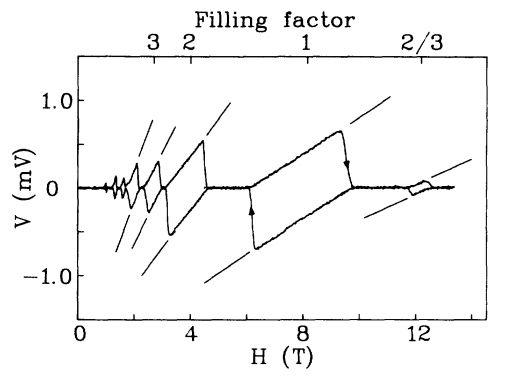
\includegraphics[width=0.7\textwidth]{figures/experimental/dolgopolov_01.png}
    \caption{Expected voltage respose in the case of time-dependent magnetic flux, it translates in an iduced electrical field (emf by Faraday) resulting in circulating eddy currets and further Hall voltages. Note that such effect is dependant of the direction of the magnetic field derivative. Figure reproduced from Dogolopov, \etal \cite{dolgopolov1992quantum}, Copyright (2022) by the American Physical Society \url{https://doi.org/10.1103/PhysRevB.46.12560}. Original caption: Potential difference between inner and outer contacts in incresing and dcreasiing magnetic field. Sample 5, \( T = \SI{25}{\milli\kelvin}\). The straight lines show slopes expected from Eqs. (1) and (2) for filling factors \( 2/3, 1, 2, 3, 4.\).  }
    \label{fig:dolgo}
\end{figure}



\subsection{Power dependance}
\label{subsec:powerDependance}

Since the thermopower is the consecuence of the temperature difference between the contacts under study, it should scale on power. 
Equation \textcolor{red}{citar equación potencia heater} states that the power at the heater will be transferred to the substrate and will produce a proportional temperature difference. In the case of the cold finger configuration one could think of radiation too, but some basic calculation of the Stefan-Boltzmann law shows that its contribution is neglegible 
\begin{equation} 
    \label{eq:stephanBotlzmann}
    \begin{split}
        P   &= \epsilon \sigma A T^4 \\
            &= (1) (\SI{5.67e{-8}}{\watt \metre^{-2} \kelvin^{-4}})(\pi(\SI{250}{\micro\meter})^2 ) (\SI{1.6}{\kelvin})^4 \\
        P   &= \SI{7.3e-5}{\nano\watt},
    \end{split}
\end{equation}
this is orders of magnitude below usual heating powers used in this work, which are avobe the \unit{\nano\watt}. In \ref{eq:stephanBotlzmann} we assume the worst case of a perfect emissivity, a larger round heater of \SI{250}{\micro\meter} radius and the worst possible base temperature.
So it is fare to assume that we transfer all heater power to the substrate, being radiation effects negligible. 

Now, such heating could or not be transferred to the 2DES. Given that our lowest temperature is around \SI{260}{\milli\kelvin}, no decouple of the electron-phonon system should be expected. Also, given the porperties of our system no pohonon focussing effects are expected \cite{anderson2012phonon,ramsbey1988phonon,karl1988imaging}. Such effects should have been observed during measurements given the variety of devices we tested, we measured Corbinos of different radius and thin, thick and Cr-doped samples, we did not find any signature of such possible efect.\textcolor{red}{inlcuir cita, también, tal vez incluir acá el detalle de las dopadas con Cr y el thinning en vez de hacerlo en el anexo únicamente.} 

Given the previous discussion, it is fare to assume that the heater power should be completely transferred to the substrate resulting in a temperature gradient in our Corbino 2DES. An then, we can expect a direct relation between temperature gradients and power applied. We show usual measured responses at different temperatures in the figures \ref{fig:D170522B_thick_power_01,fig:D170522B_thick_power_02,fig:D190130A_Cr_power,fig:F150709B_power_01,fig:F150709B_power_02}. Unless stated, all measurements will be standard, in the sense that our usual magnetic resolution measurements were \SI{10}{\milli\tesla}.

\textcolor{red}{Juntar las imágenes de potencia en tres paneles (uno por muestra) y mejorar los tamaños de letra. Hacer uno específico para la zona de los LL. Tal vez usar directamente el que pusimos en el paper y que va en modeling.}

\begin{figure}
    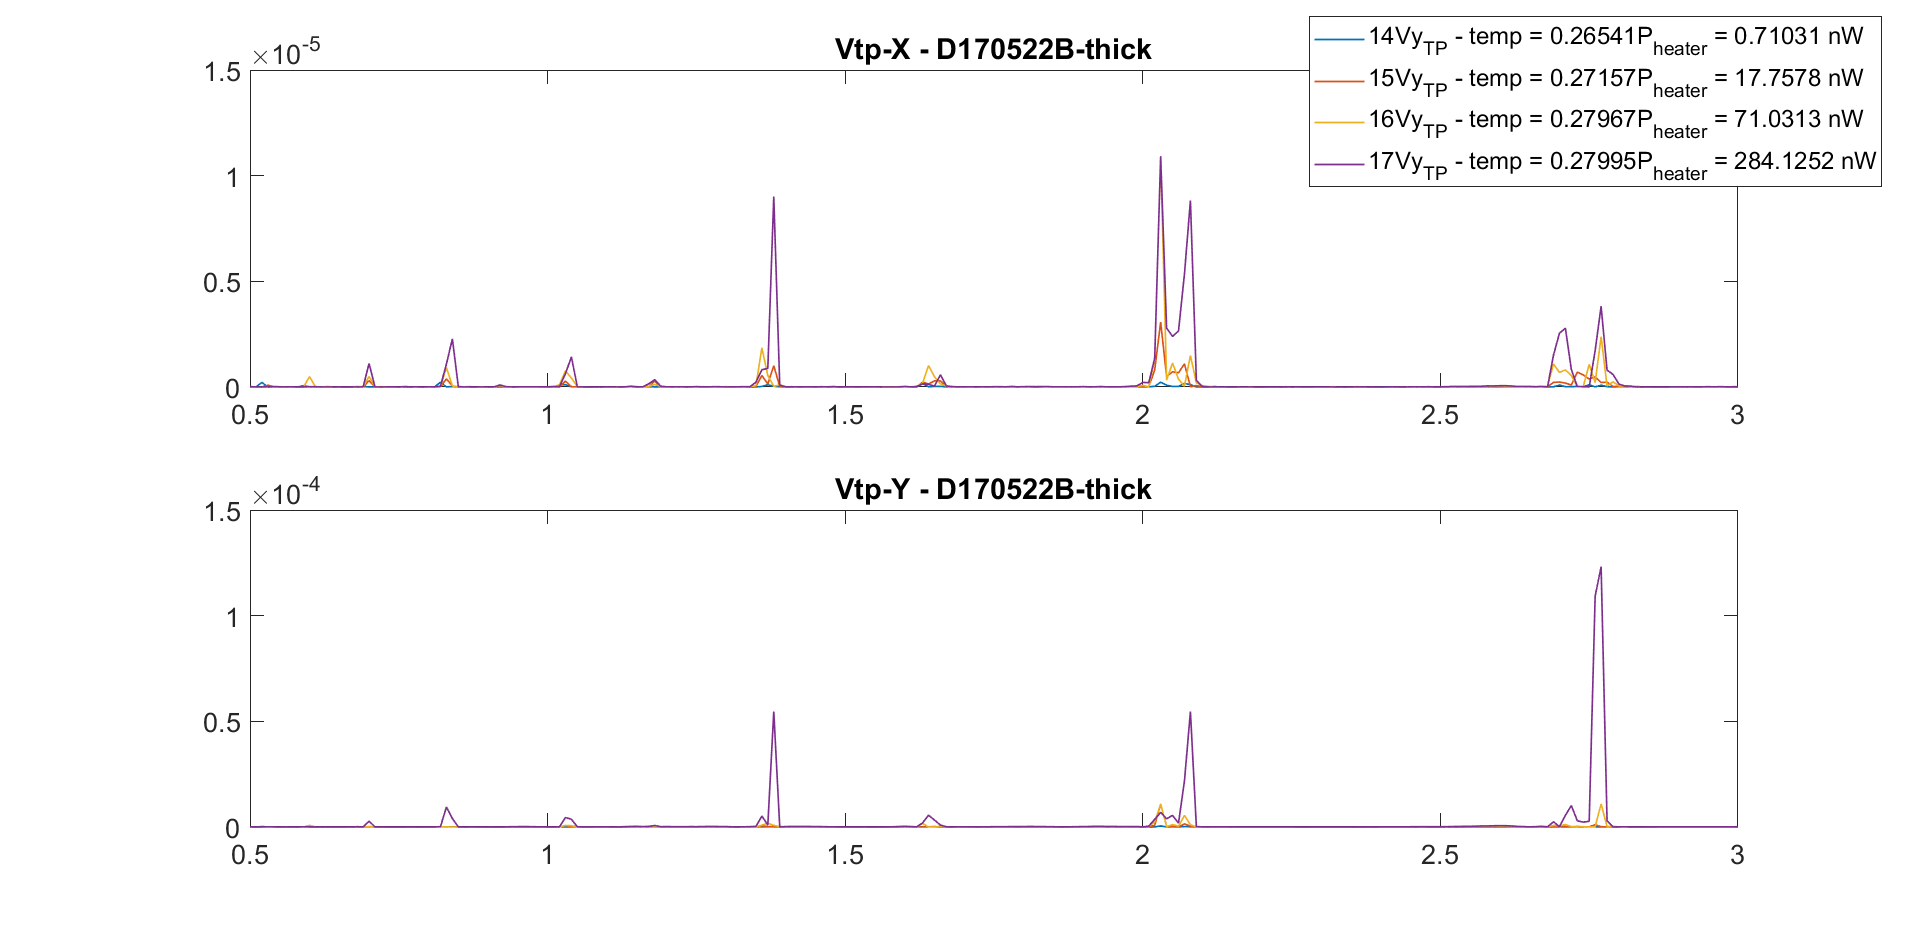
\includegraphics[width=1\textwidth]{figures/experimental/powerDependance/D170522B-thick-cambio-potencia-01.png}
    \caption{caption.}
    \label{fig:D170522B_thick_power_01}
\end{figure}


\begin{figure}
    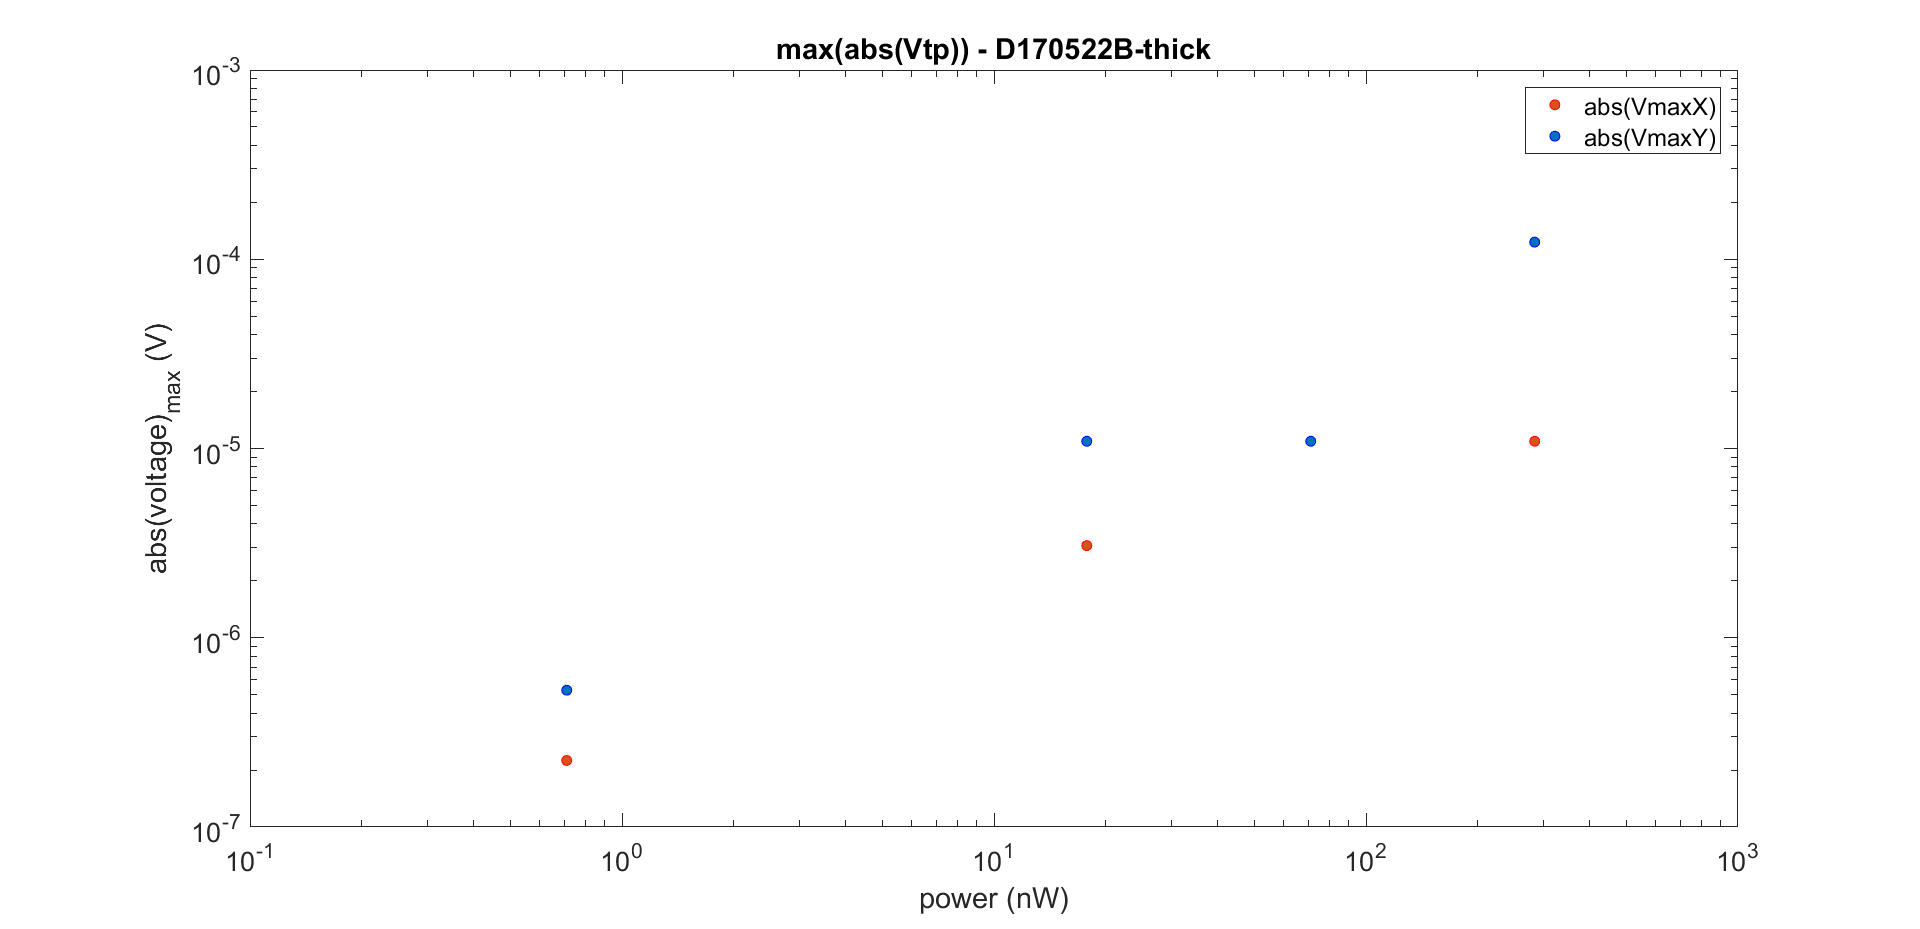
\includegraphics[width=1\textwidth]{figures/experimental/powerDependance/D170522B-thick-cambio-potencia-02.png}
    \caption{caption.}
    \label{fig:D170522B_thick_power_02}
\end{figure}


\begin{figure}
    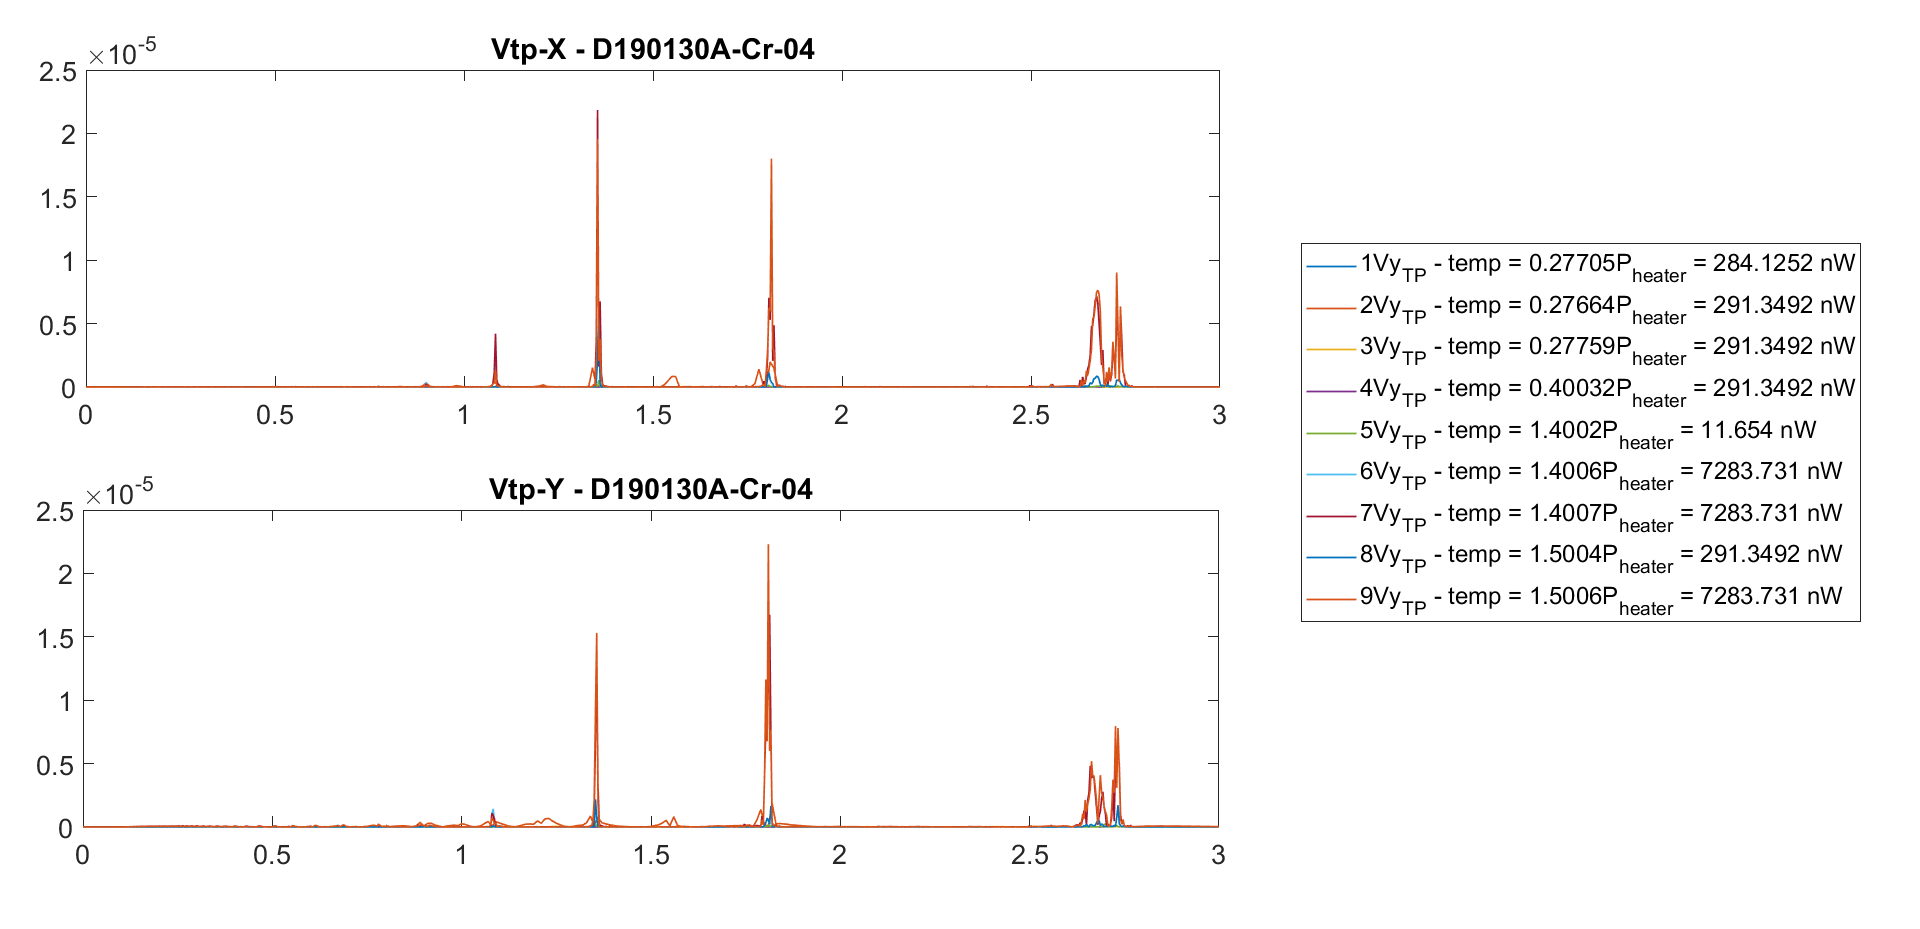
\includegraphics[width=1\textwidth]{figures/experimental/powerDependance/D190130A-Cr-04-todas.png}
    \caption{caption.}
    \label{fig:D190130A_Cr_power}
\end{figure}


\begin{figure}
    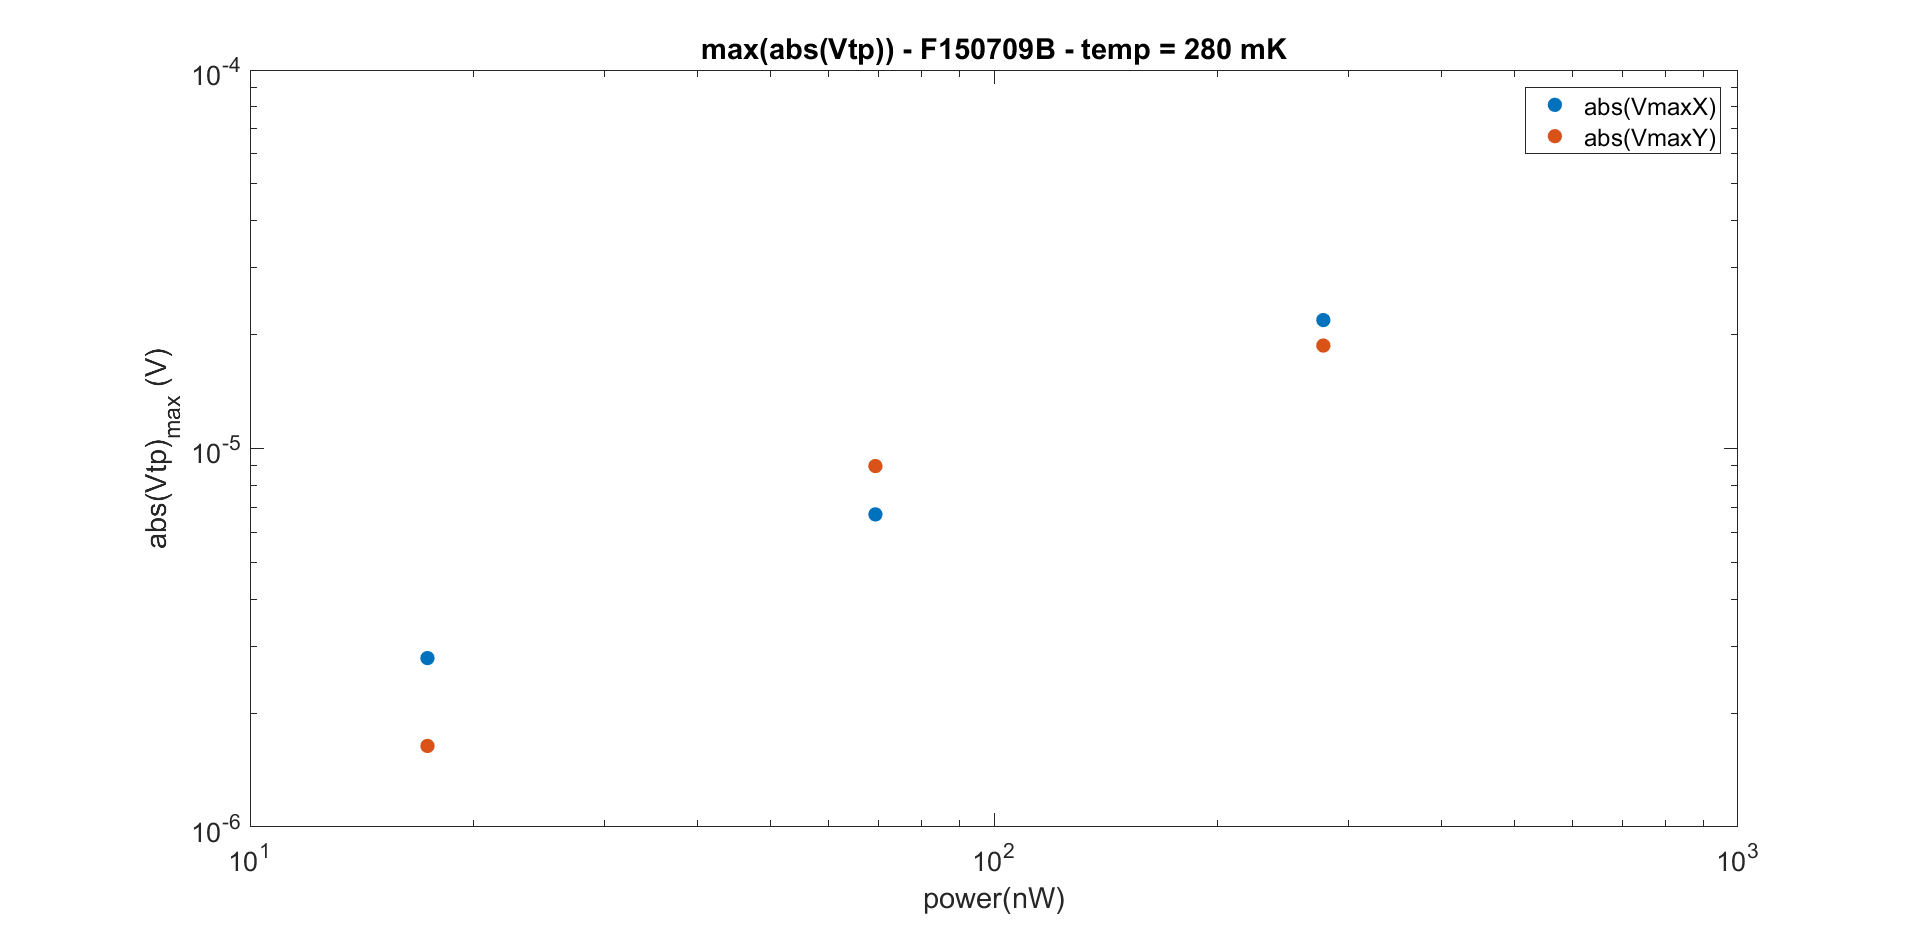
\includegraphics[width=1\textwidth]{figures/experimental/powerDependance/F150709B-cambio-potencia-01.png}
    \caption{caption.}
    \label{fig:F150709B_power_01}
\end{figure}

\begin{figure}
    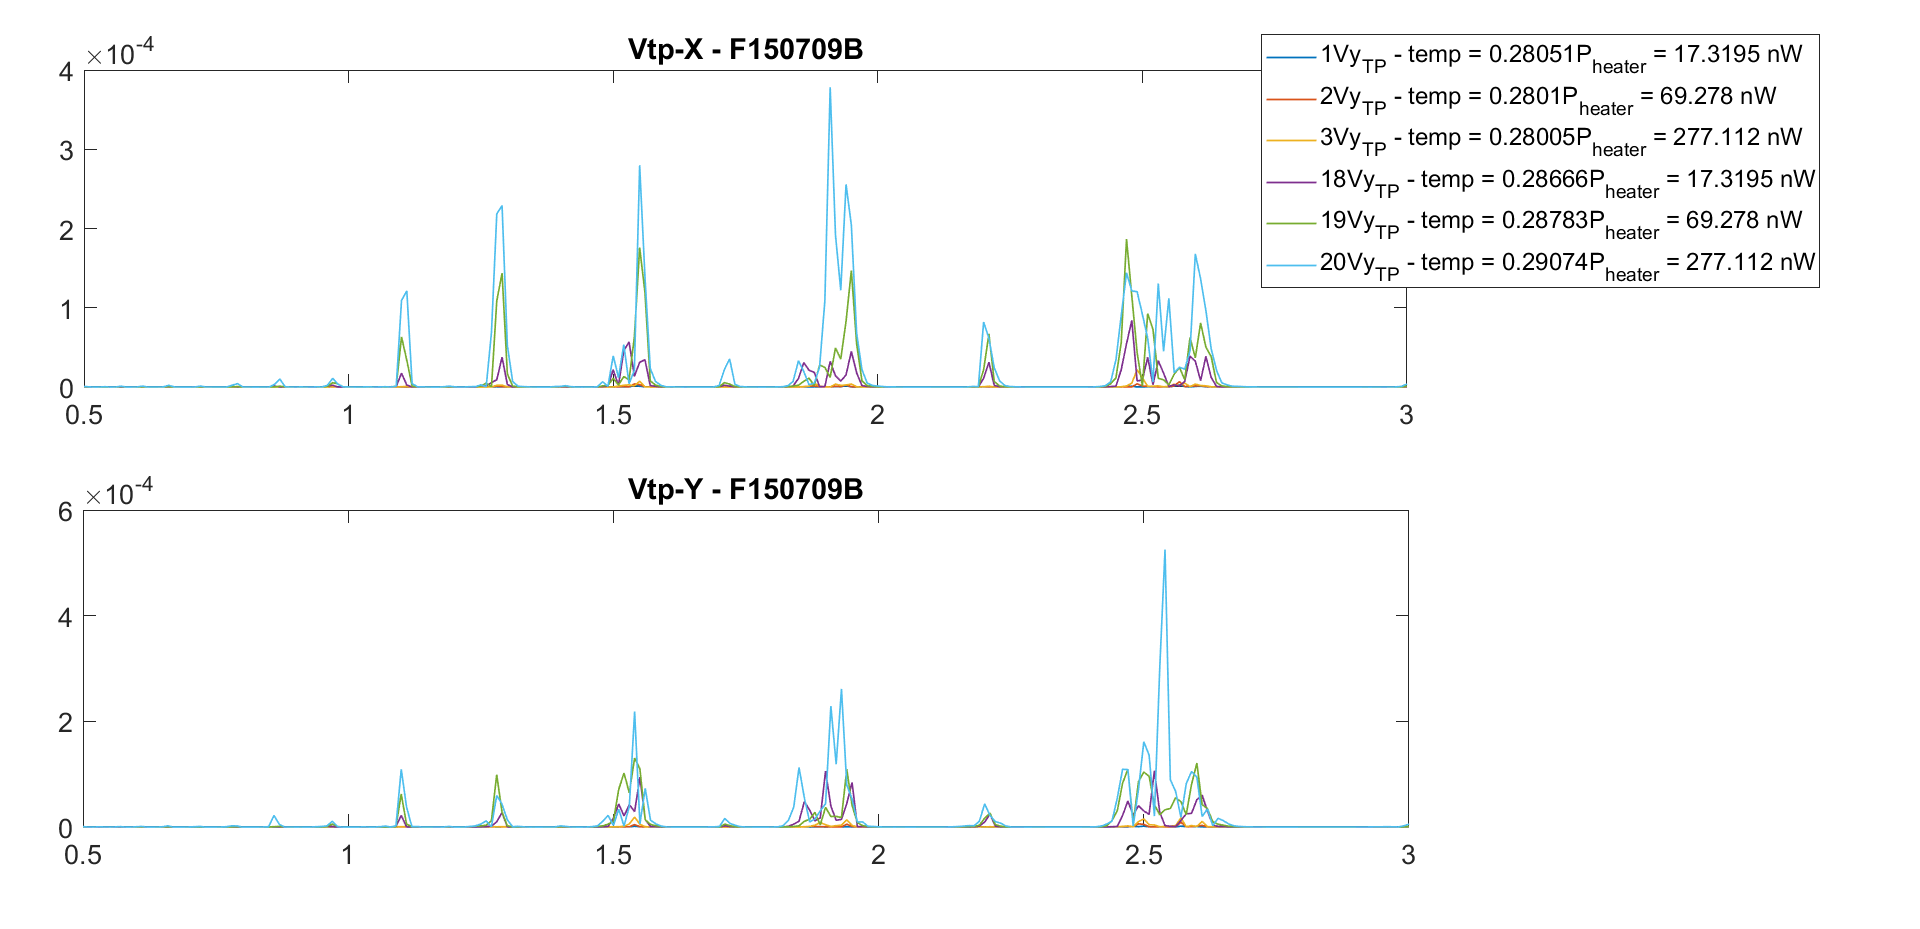
\includegraphics[width=1\textwidth]{figures/experimental/powerDependance/F150709B-cambio-potencia-02.png}
    \caption{caption.}
    \label{fig:F150709B_power_02}
\end{figure}

As shown, in all cases the response of the system depends on the power applied, as expected. What was not expected is the huge response in the gap, here shown in the \( \vtpx \) plots, that scales as the one of \( \vtpy \) in the gap. We shall come back to this in \textcolor{red}{citar la sección donde se discute esto.}. We will come back to the power dependance in \textcolor{red}{citar ch:modeling, fig: power dependance con modelo}, where whe show how the developed model predicts the different responses at different heater power.


\section{Thermovoltage and conductance measurements}

Up to now we have discussed some aspects of the measurements but not in detail, we shall do it in this section. Coming back to the experimental setup already mentioned, let us discuss two main measurement situations initially: a- conductance measurements, and b- thermopower measurements. 

\begin{figure}
    \centering
    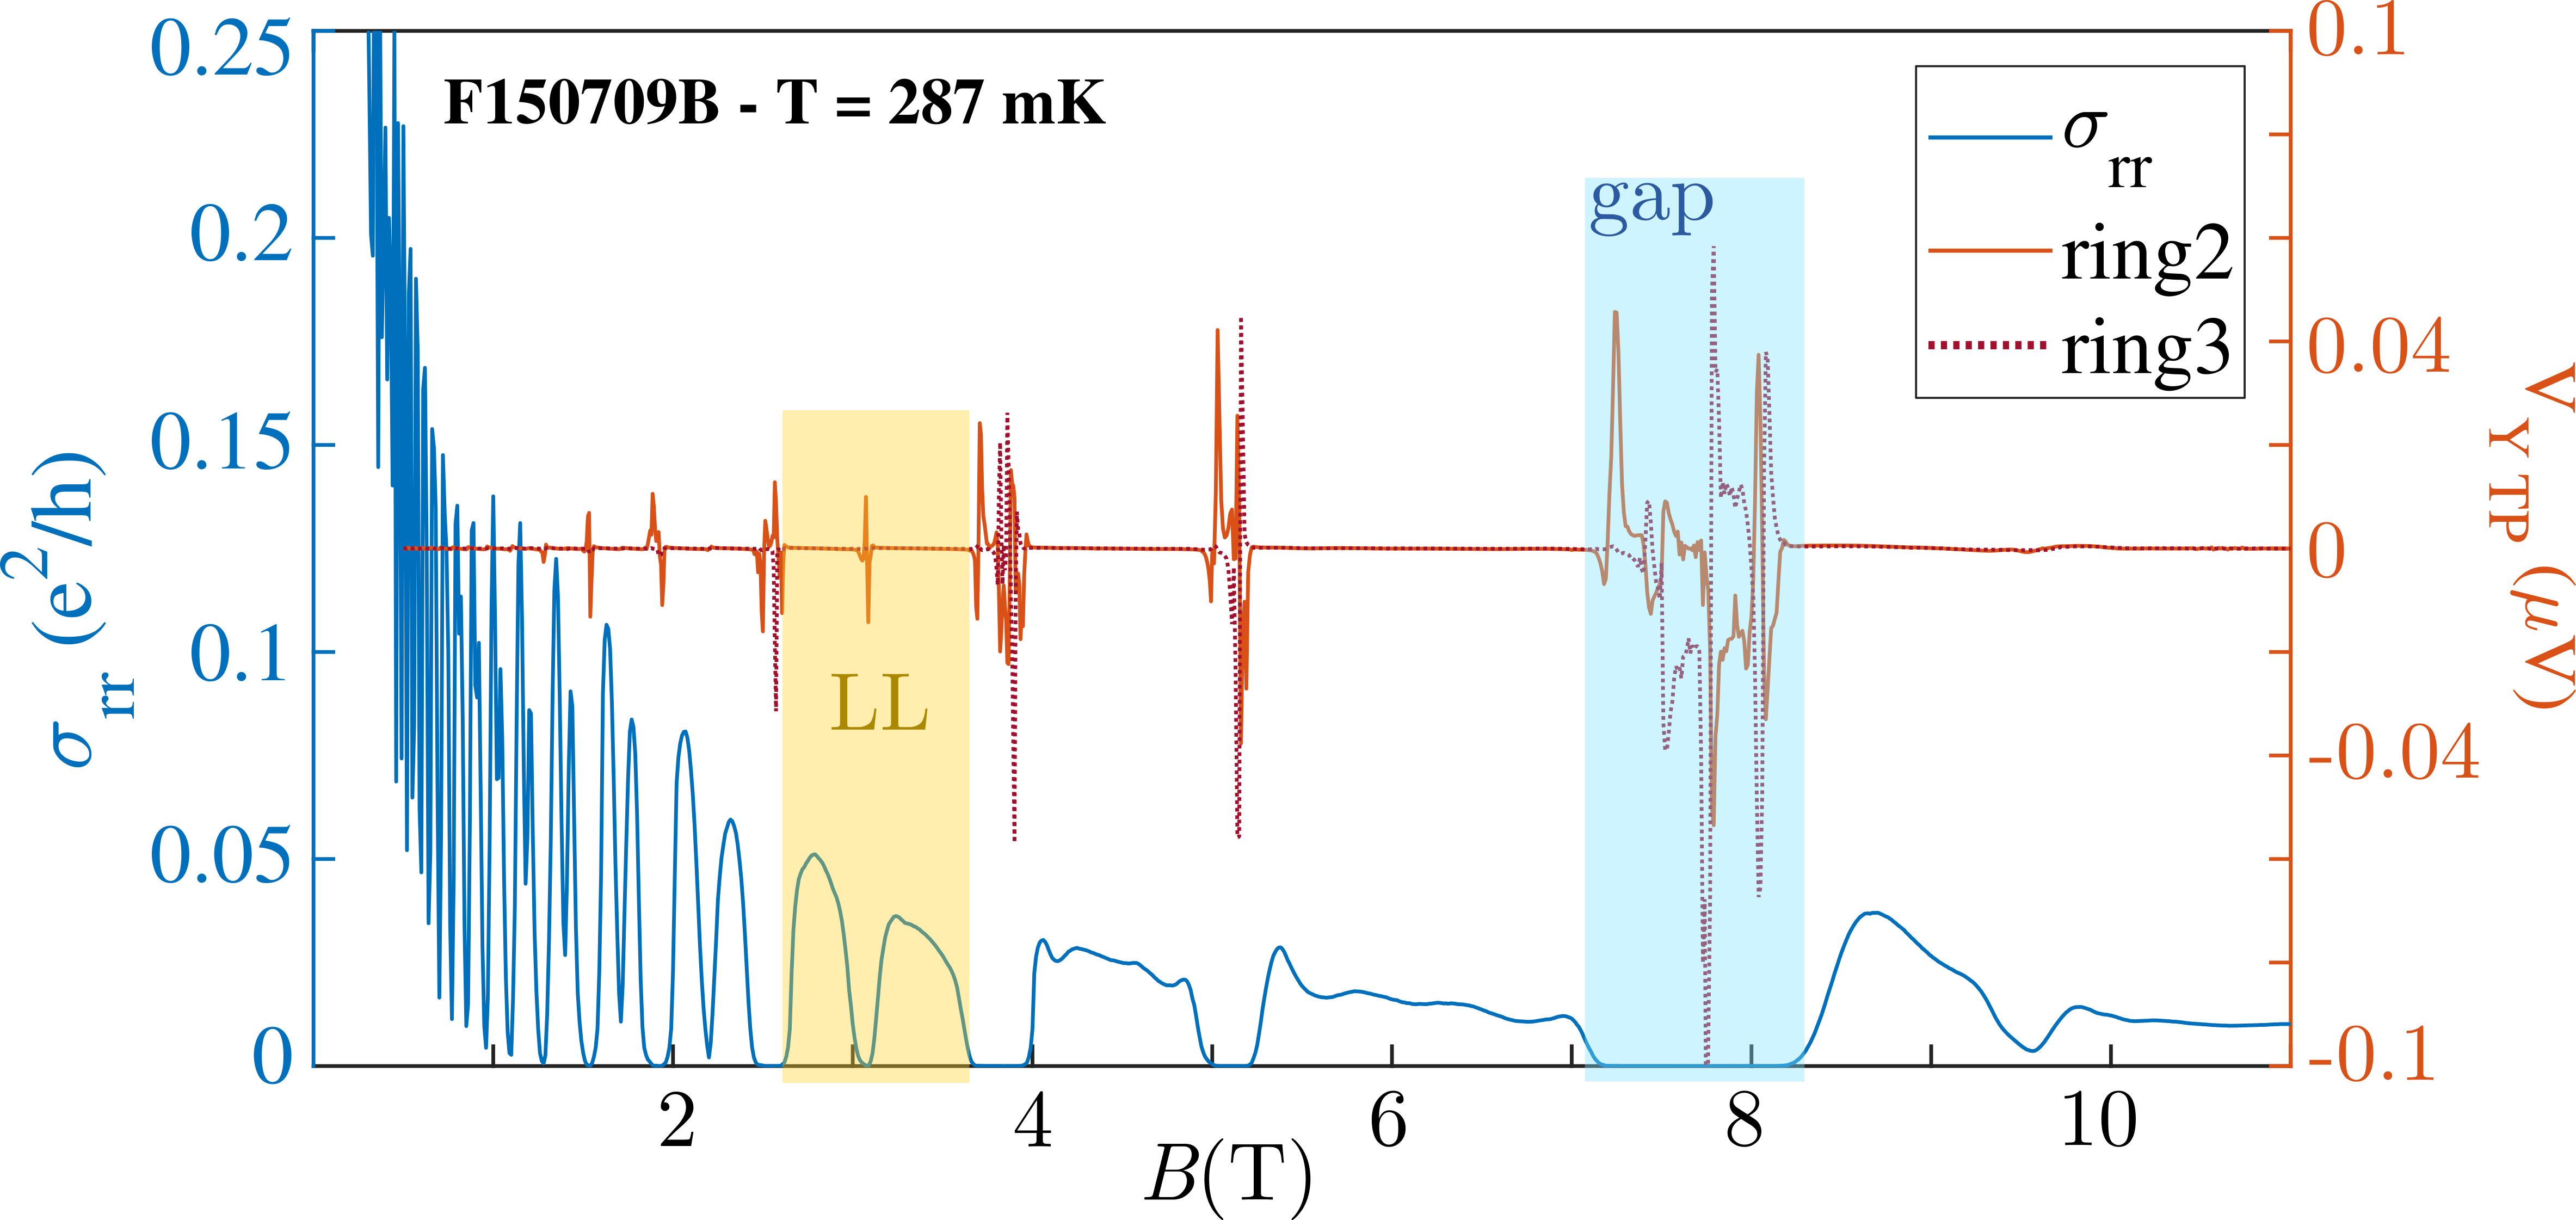
\includegraphics[width=1\textwidth]{figures/experimental/GandVtpExample.png}
    \caption{This is a typical conductance example, showing the expected behavior of the system in its different stages (LL and gap). A very schematic measurement inset is given, the actual measurement set-up is given in Fig. \ref{fig:corbino_exp_setup} \textcolor{red}{No puse los filling factor, agregar, también los N de los LL y el spin (ver el grafico del paper de corriente).}}
    \label{fig:GandVtpExample}
\end{figure}

Figure \ref{fig:GandVtpExample} shows some typical results of the conductance (blue curve) and of the \( \vtpy \), orange and reddish curves for ring 2 and 3, we introduce here this measurements to introduce to some particularities and be able to discuss later in detail the different details they have. 
In this measurements, as we increase the magnetic field the Subnikov de Haas (SdH) oscillations develop, until quantization ($G = 0$) is reached. Each bulb in this curve is the result of the different Landau levels, and as the magnetic field reaches higher values ($B \sim \SI{1}{T}$) full quantization is obtained and so the mobility gap completely displayed by the conductance (conductivity in this plot). Also, it is important to note the point at which the spin splitting of the system can be observed ($B \sim \SI{1.5}{T}$ for this sample and temperature). This is why the LL in yellow is marked over two conductance increases, they belong to the same LL but having different spin. This measurements were produced by applaying a voltage to the inner ohmic contact of ring 2 while measuring the current circulating at the outer contact 
\textcolor{red}{tal vez conviene nombrar cada contacto con un número y hacer un gráfico.}
by means of the I/U amplifier locked to the excitation voltage at a frequency $f = \SI{113}{\hertz}$. 

Most measurements in this work will focus in the region \SIrange{0.5}{3}{\tesla}, because the measurements were very time consuming, for example figure \ref{fig:GandVtpExample} required an overnight measurement for $G$ and a complete day for $\vtp$. Also, we wanted to avoid the inclusion of FQHE effects on this stage of the developments, since many more possible effects could become relevant.

Regarding the $\vtp$  measurements in Fig. \ref{fic:GandVtpExample}, it was not expected that the system presented such large and complex behavior in the gap. Another point (not shown in this figure) is that the out of phase response in the gap was of the same magnitude as the one shown, another unexpected result that we shall discuss in the next chapter. Also note that ring 2 and 3 are consecutive and the change in sign, this are floating measurements, so there can be a change (overall phase) modifying the output. 


We performed measurements at INTI and at ETH-Zürich (Prof. Wegscheider's group), the measurements set-ups at each location was different, depending on the equipment availability. In the case of INTI, we use a wet $^3$He cryostat while at ETH we performed measurements in a cold finger configuration, further instrumental details are given in \ref{appendixc}. This is a conceptual difference from the thermovoltage and temperature measurement point of view, in the foremost the He bath may impact in the power dissipation and of the heater and the temperature achieved by the system. It also sets issues regarding how to apply the temperature approach we describe in \textcolor{red}{citar temperature meas section}. These issues are not present in the cold finger configuration, where the heat is almost exclusively transmitted by conductance. 
A COMSOL simulation using typical properties of GaAs (\url{http://www.ioffe.ru/SVA/NSM/Semicond/GaAs/}), including the He liquid and thermal fixed edges to the sides of the sample and a large base temperature of \SI{1}{\kelvin} shows that, even with our wet cryostat, we can expect a heating profile of several \si{\milli\kelvin}, as shown in Fig. \ref{fig:comsolHelium}.


\begin{figure}
    \centering
    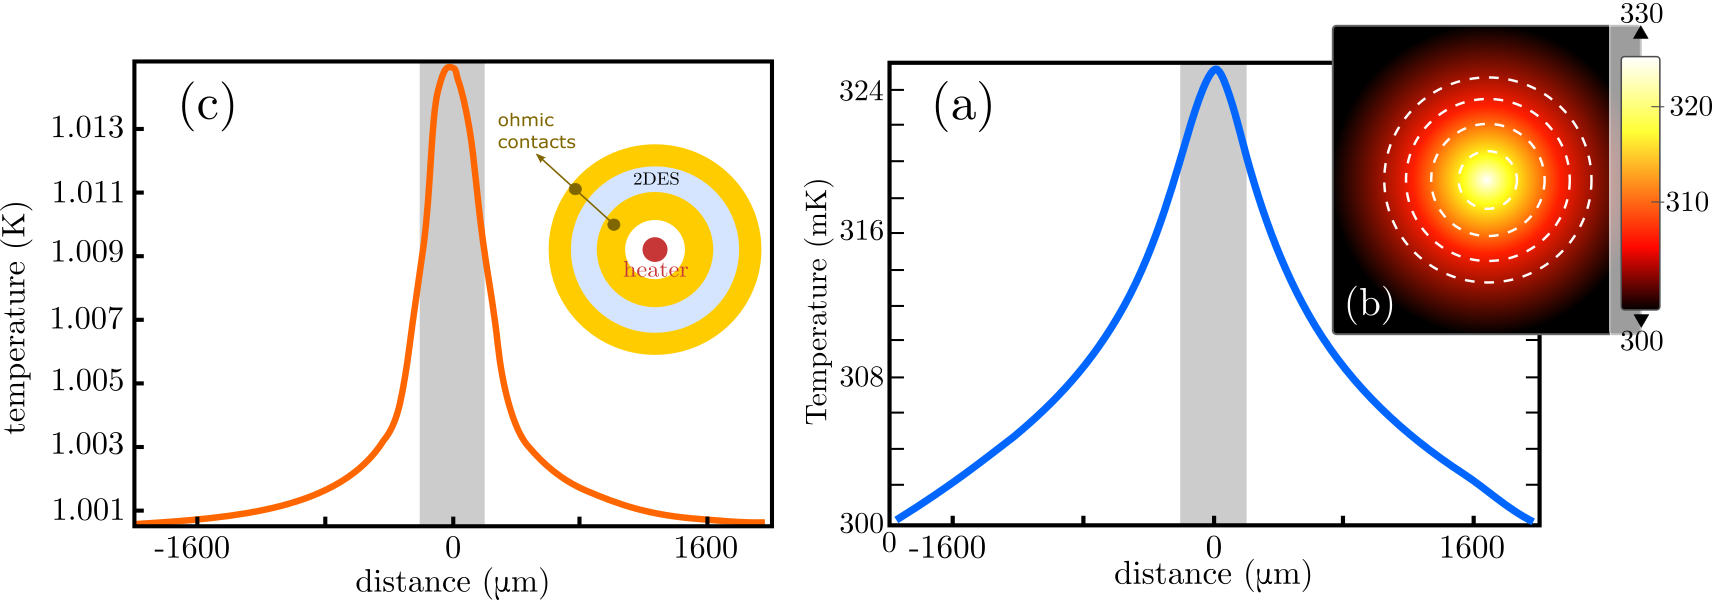
\includegraphics[width=1\textwidth]{figures/experimental/comsol_helium_dry_and_wet.png}
    \caption{Simulation of both (c) wet and (a) dry systems, it is assumed that a a point heater induces a power on a GaAs crystal. The borders of the sample are anchored in both cases. But in the case of the wet system the Helium thermal conductivity is also included. Possible radiation is discussed in the text. Gray area indicates the etched central mesa area in the samples. (b) shows a 2D profile of the expected temperature.}
    \label{fig:comsolHelium}
\end{figure}


\textcolor{red}{tenemos algunas mediciones de INTI que sería interesante incluir, pero va a volverse todo largo y no las utilizamos en las publicaciones. Lo que aprendimos acá nos ayudó a llevar a cabo las medicones allá y configurar los equipos de forma correcta. No sé cuánto incluir de esto y si tiene sentido o no. Personalmente creo que es bueno indicar al menos las cosas que no funcionan para que otro se salve de probarlas, o incluso las pueda llevar acabo con mejoras.}

As we have said the thermovoltage measurements are well defined when we use an ideal (infinite) input impedance. In the case of the LL, when the system is acting basically as a metal, it should be enough to use some standard measurement configuration. But, once we reach quantization, i.e. when measuring in the gap, the impedance becomes a much important deal. In the gap, the system presents an almost null conductance, in the order of \textcolor{red}{meter valor conductance}, to overcome this problem several configurations were tested resulting in the use of the differential DC amplifier sketched in the setup of Fig.~\ref{fig:corbino_exp_setup}, also a picture is given in Fig. \ref{fig:DCamp}. This is a fixed $\times 1000$ differential amplifier developed specifically for very accurate low noise voltage measurements \cite{Maerki2017}. This instrument had two inputs per channel (top  connectors), so a maximum of two signals per thermovoltage run could be measured. Then two $\times 1000$ amplified output channels are provided (OUT 1 and 2). We will not describe it here but is a very interesting device as explained in its describing work \cite{Maerki2017}. 

\begin{figure}
    \centering
    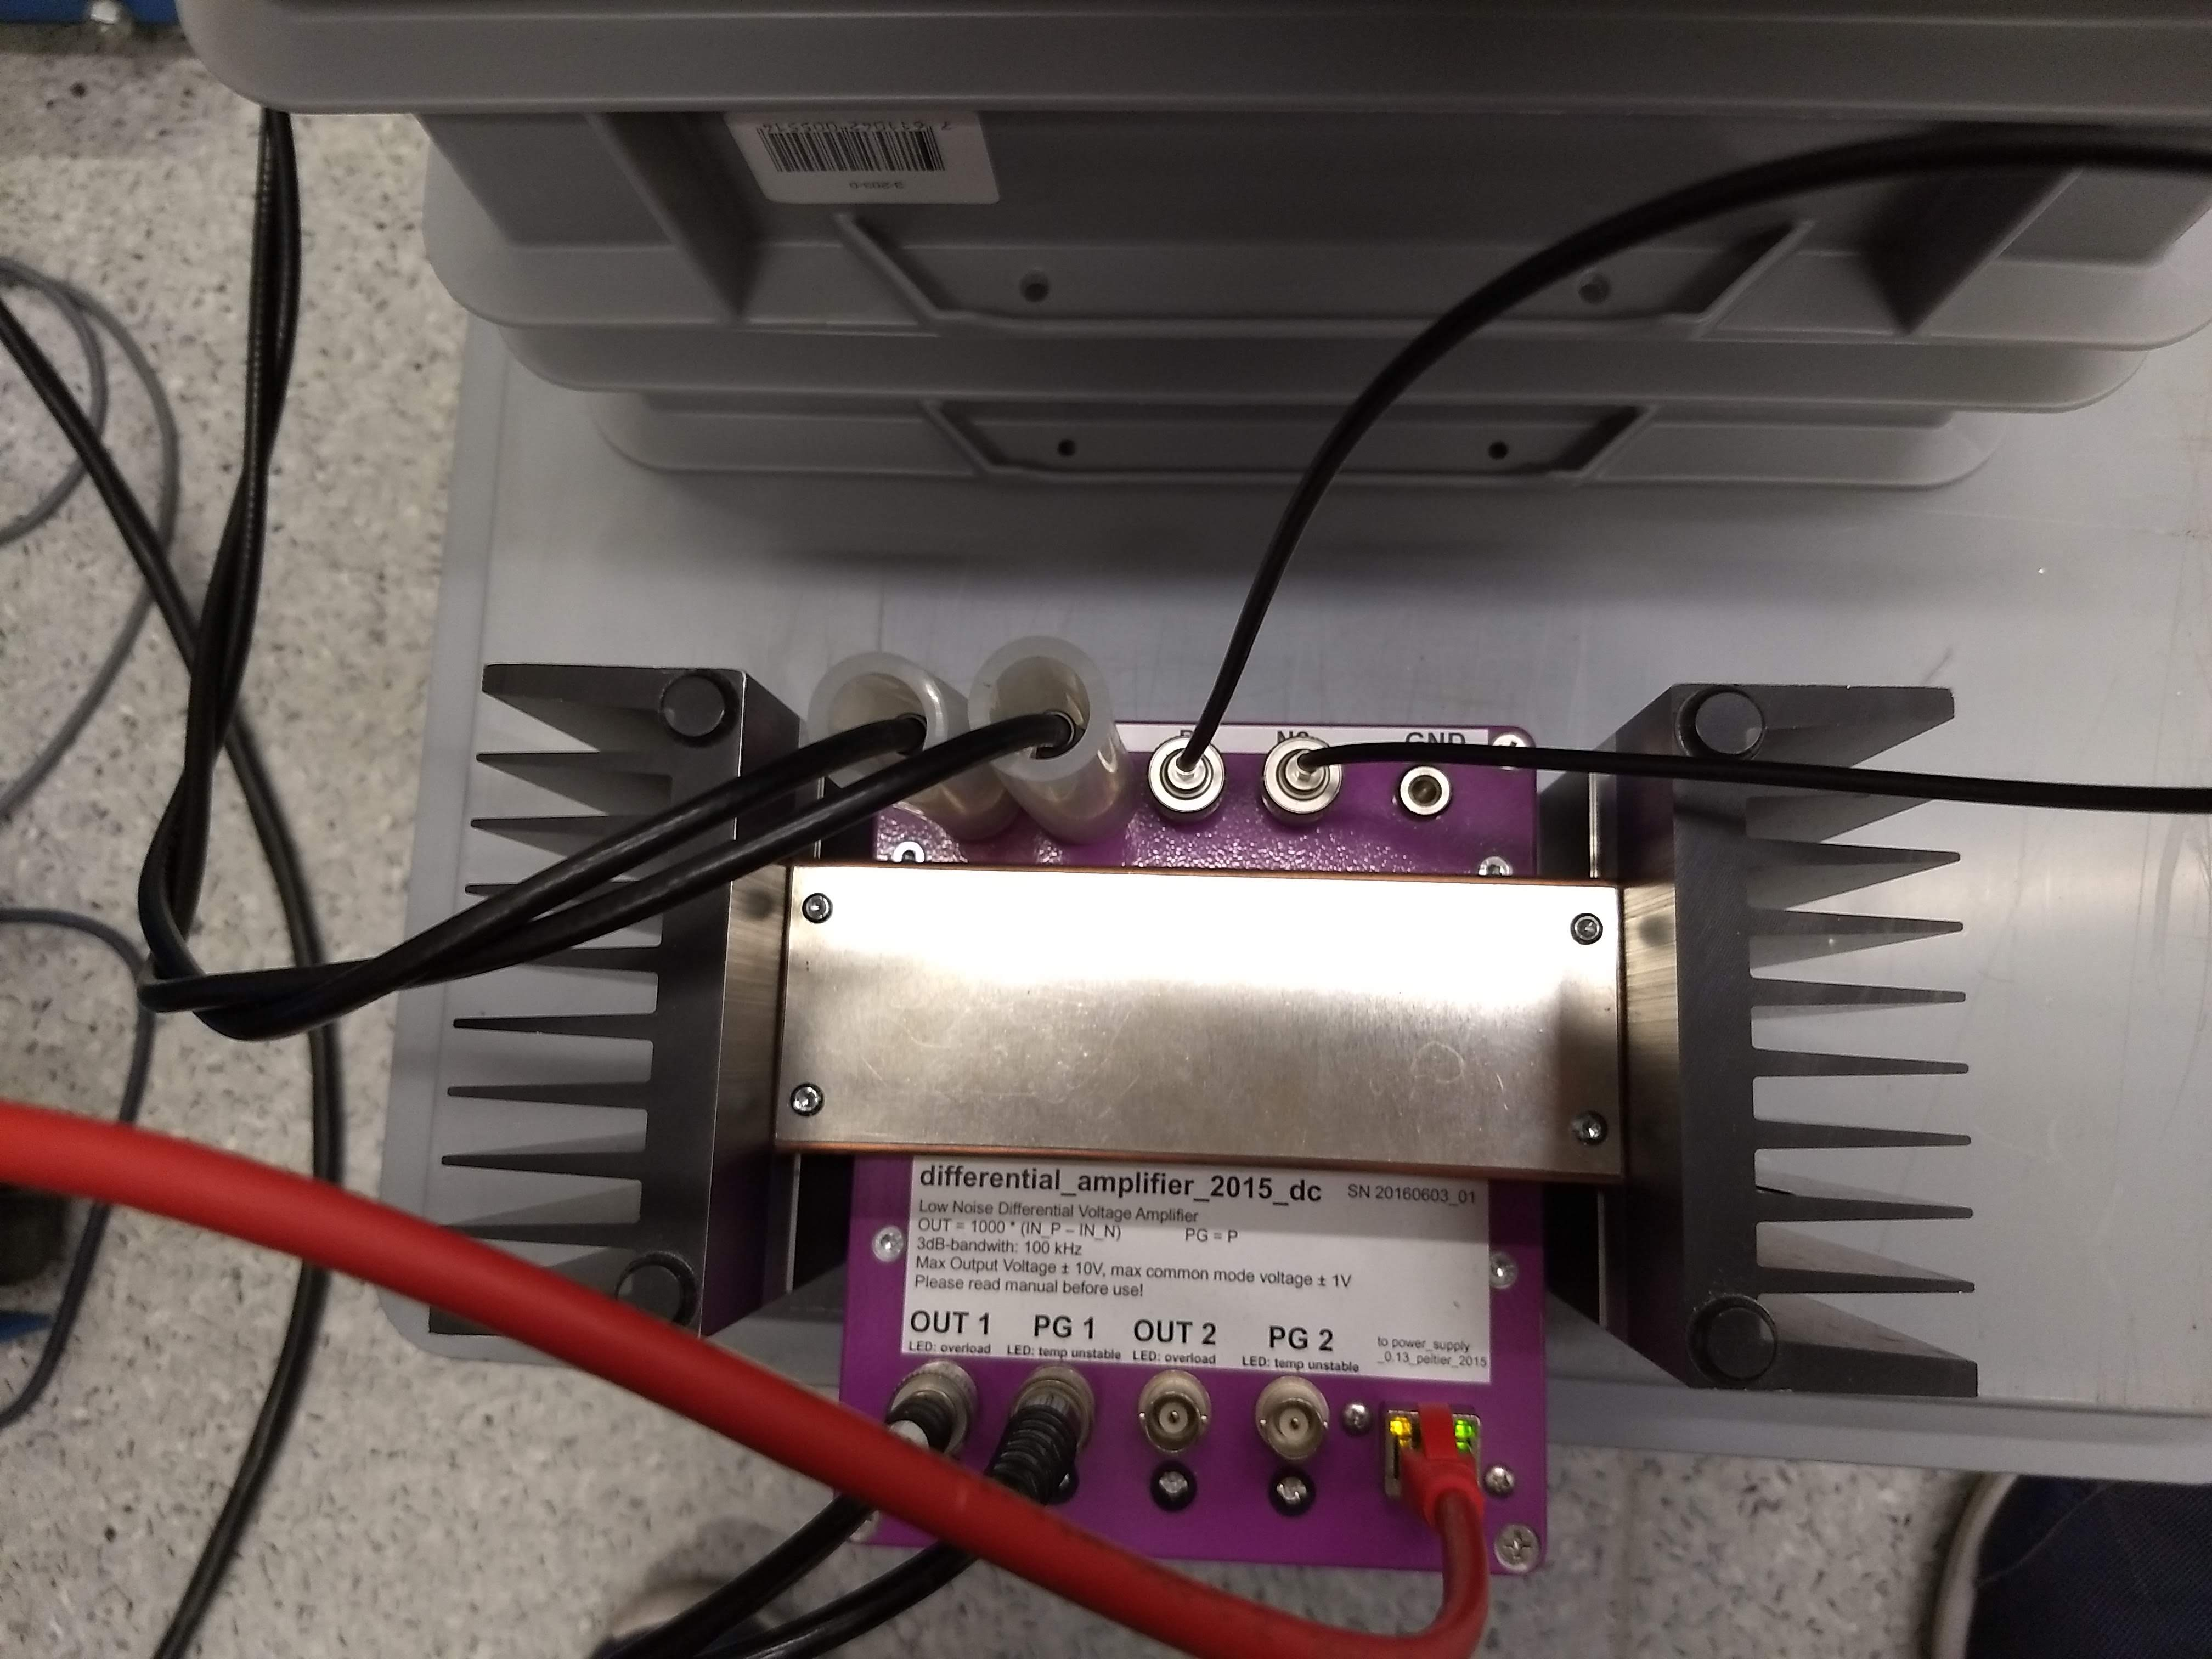
\includegraphics[width=0.6\textwidth]{figures/experimental/DCamp2.jpg}
    \caption{Image of the DC amplifier used for the  \( \vtp \) measurements. The use of BNCs is not the best approach, but it was the standard used in the laboratory. Note the protection in the input (left) terminals, this avoids thermal currents and possible touching to modify the voltage measurements. 
    The PG outputs allows to measure the one of the inputs to the internal amplifier, finally the RJ45 is the power input.  \textcolor{red}{esto último no sé si es necesario incluirlo, es detalle que usé pero no describo más.}}
    \label{fig:DCamp}
\end{figure}

Given the characteristics of this device it is possible to measure up to \SI{1}{\kilo\hertz} without affecting its performance. 

Many measurement runs were performed to the devices using the configurations described in this chapter. We will return to them in \ref{ch:modeling} in a data driven approach, we shall discuss there our model and how it relates to the measured responses of the different devices. 

\chapter{Temperature gradients determination}
\label{ch:temperature_corbino}

Up to this point we have described how we measured the thermopower and conductance of the system, we also introduced the theory to describe them and the effects we aim to exploit, we shall use in the next section to model the system. From this modeling we will obtain a temperature gradient $\Delta T$, responsible of the behavior of the thermopower. So we need a way to measure the electronic system temperature, here we introduce method to do so, which is of main importance to the objectives of this thesis.

The first type of measurement one could think of is to include somehow a set of  \textcolor{azulGris}{\textbf{resistive sensors}}, thermally attached to the devices. The advantage being that they are well developed and in common use in cryogenic technologies. But, they are integrating systems, the measurement is through thermal contact so, the actual temperature measurement have to be done having several resistive sensors attached to different positions (inner outer ring) of our Corbinos, i.e. 8 sensors, 16 or 32 cables (if 4 point probing is used), meaning a complete rewiring of the probes. The actual measurement would not be of the electronic system, but an approximated value given by the crystal. 
Also, a very good electric isolation had to be obtained, otherwise the thermopower measurement would be compromise. 
The sensors should have to be glued to the devices, even with the best approach would include tensions to the crystal, resulting in a modified thermopower profile.
Because all of this, this type of arrangement was discarded.

\begin{figure}
    \centering
    \includegraphics[width = 1\textwidth]%
        {figures/temperature_corbino/probe-diagram.png}
    \caption{Dry cryoprobe images. \textit{Top left:} note the position of the temperature sensor. This sensor is the one mentioned over the thesis. Samples are mounted from below, as seen in the \textit{top right} images. Other details fo the cryoprobe can be seen in the bottom images, particularly the $^3$He heat exchange, the $^4$He pick-up line, between others.}
\end{figure}

We could also think to produce an absolute temperature measurement setup based on \textcolor{azulGris}{\textbf{Johnson noise thermometry}} \cite{Johnson1928, nyquist1928,webb1973noise,qu2019johnson}. 
In our case this would mean to set some way to thermally attach our Corbinos to such measurement system. 
It would be an approximate measuring setup, measuring each Corbino ring, approximating $\Delta T$ as a temperature difference between them. 
This type of measurement would imply to produce the measurement cryo-circuits, and probabbly would need some kind of switching system to detach its electrical connections during the thermopower and conductance measurements, not an easy task. 
This kind of measurement is absolute and reliable, but its technology and components were not available in our systems. 
Once again, given the problems described we aimed for a different approach.

From Kobayakawa, et. al \cite{kobayakawa2013diffusion} we have another temperature determination option, but implies to use also their RF measurement configuration, we could not use our heater approach.

\textcolor{azulGris}{\textbf{Temperature by conductance measurement:\\}}
Finally, since the conductance response is dependent on the temperature of the electronic system one could think of using it as temperature sensor. This is what works by Chickering et al. \cite{chickering2010thermopower}, Liu et al. \cite{Liu2018} and Endo et al.\cite{endo2019spatial} have used. They measure the thermal conductance in a Hall bar configuration to obtain a temperature for the system. 
In these cases they infer such temperature by equalizing the temperature of the system to the one of an included heater. 


We make use of such idea and take advantage of the conductance change for different powers and base temperatures, from which we are able to set a temperature gradient function, dependent of the power applied and the base temperature of the system. This approach avoids the need to include a glued sensor, for example, which would introduce problems such tensions in the crystal, extra thermal impedance, problems regarding its position, among others.

\begin{figure}
    \centering
    \includegraphics[width=0.7\textwidth]%
        {figures/temperature_corbino/experimental-setup-calTemp.pdf}% picture filename
    \caption{%
    (a) Experimental setup of the temperature calibration procedure. The $V_{\mathrm{h}}(f_\mathrm{h})$ bias voltage (red) generates the desired power $P$. Meanwhile, the conductance is measured in the innermost (1) and outermost (4) Corbino rings through a current to voltage converter. In this case we also have the possibility to make DC (DMM) and AC (LIA) measurements, biasing the Corbinos by means of voltage $V_{\mathrm{in}(f_{\mathrm{in}})}$ determined measuring the voltage divider output (black). \\
    Note that there are two different frequencies here, one to produce the thermal gradient as in the thermopower $f_{\mathrm{h}}$. A second one $f_{\mathrm{h}}$ is use for the conductance determination.\\
    (b) Corbino device AA section cut. Here the bottom drilled hole avoids thermal transfer from the substrate, for the same reason, it is only photo resist (PR) glued on one side.
    }
    \label{fig:calTempExpSetup}
\end{figure}

The final experimental setup it is shown in Fig. \ref{fig:calTempExpSetup}, we apply a voltage $V_{\mathrm{h}}(f_\mathrm{h})$ to the heater, resulting in a dissipated power $P$, red circuit in Fig. \ref{fig:calTempExpSetup}. Meanwhile a second bias is applied to the innermost (1) and outermost (4) Corbino rings (black circuit). So, the current circulating in the Corbino is measured by means of the circuits and instruments shown in green, resulting in a conductance measurement. 

There are several possible approaches to the heater and Corbino bias, one could use a DC, AC or a DC$+$AC signal. Several alternative configurations were tested. Just to mention one, we tried to use a differential signal generator, so a square wave would be used in different fashions, but the resulting measurements were not satisfactory, noise, grounding among others, impeded its implementation.

We finally used the following protocol (settling times are not listed):
\begin{enumerate}
    \item Set the minimum possible base temperature of the cryostat $T_{i=0}$.
    \item\label{enum:field} Set a magnetic field $B_{\nu_0}$ in an almost developed conductance minima  (almost zero), set the magnet to persistent mode. The field selected ensures that any small change in temperature shall produce a significant change in conductance.\footnote{This means that we are using odd filling factors, they are the first to break.}
    \item\label{enum:zeroPower} Measure the conductance $G\left( B_{\nu_0}, T_0, P_0 = \SI{0}{\nano\watt} \right)$.
    \item\label{enum:tempCal} Produce a set of different conductance measures $G\left( B_{\nu_0}, T_0, P_j \right)$ at different heater powers $P_j$.
    \item Increase the base temperature $T_i$.
    \item Repeat 4 and 5 until no power change can be obtained, resulting in a set of $G\left( B_{\nu_0}, T_i, P_j \right)$.
\end{enumerate}

\begin{figure}
    \centering
    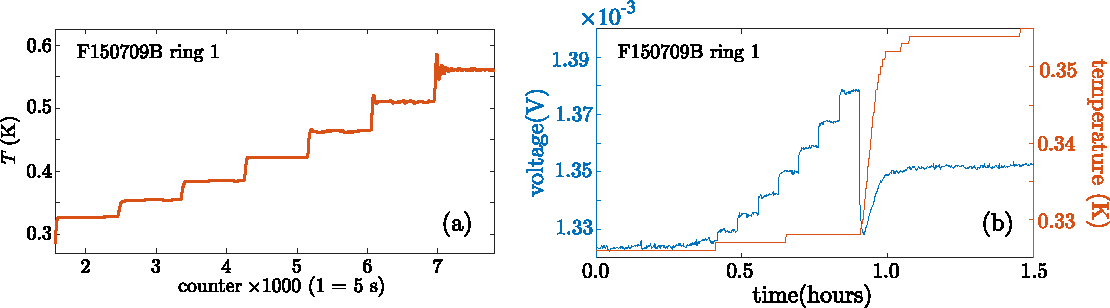
\includegraphics[width=1\textwidth]{figures/temperature_corbino/DCresponseVoltageTempCounter.pdf}
    \caption{Unprocessed measurements of the (a) temperature and (b) voltage response of the system for the same sample and ring. In (a) a set of base temperatures at $P_0 = \SI{0}{\nano\watt}$ was programmed. Figure (b) shows the system response for a set of powers $P_j$ at a specific temperature $T_i$, at  $t \approx \SI{0.9}{\hour}$ an automatic change is produced, the power is again set to zero and a new temperature $T_{i+1}$ established.}
    \label{fig:DCvoltTempCounter}
\end{figure}

A typical temperature measurement it is shown in Fig.~\ref{fig:calT}. Figure \ref{fig:DCvoltTempCounter}(a) shows the system response while changing the base temperature $T_i$. Note that for the lowest temperatures the controller is able to reach easily the set temperature, while once higher settings are placed the system overshoot and a small oscillatory transient must be overcome. This process is time consuming, and the final temperature could change from different runs, this is why we decided to produce the power change measurements once the temperature was reached. This is shown in Fig.~\ref{fig:DCvoltTempCounter}(b), here a set of DC powers $P_j$ was programmed and the temperature and voltage (i.e. current then conductance) was obtained. At time $t \approx \SI{0.9}{\hour}$ the DC heater power is set to zero and a new cold finger temperature established, such change in temperature determines a change in the  conductance minima this is why the voltage changes. After $t = \SI{1.5}{\hour} $ a new set of power changes is made (not shown in this figure). 

Regarding the selected magnetic field position $B_{\nu_0}$ mentioned in item \ref{enum:field}, we could also use the side near a fully quantized filling factor \cite{chickeringPhD}, but the resolution resulted to be lower. Also, when making step \ref{enum:zeroPower} we indicate $P = \SI{0}{\nano\watt}$ but we are actually using the lowest possible configuration of the LIA, $V = \SI{4}{\milli\volt}$. The only way to apply zero power in our setup is to disconnect or short circuit the interconnection box, see Fig.~\textcolor{red}{CITAR FOTO INTERCONEXION BOX}, but this would prevent any automation possibility. We have checked that such minimum voltage (heater power) is below the measurement resolution, even for the thermovoltage measurements, so we can assume it to be zero power.

Finally we obtain a set of calibration curves like the ones shown in Fig. \ref{fig:calT}, for the innermost (ring 1) and outermost (ring 4) rings. Colors correspond to a different powers, each point in this figure is the result of the statistics of 20 measurements once the system stabilizes, after each temperature and power change, see Fig. \ref{fig:DCvoltTempCounter}.  

We want to be able to experimentally determine the temperature gradient on the sample. In order to do so, an interpolation $f(T, G, P)$ is made, from which it is possible to determine a $\Delta t (G) = f^{-1}(G,P)$. To further discuss this approach, say we look at point \textit{a} marked in Fig. \ref{fig:calT} at $T \approx \SI{260}{\milli\kelvin}$ and $P = \SI{277}{\nano\watt}$, we can think of it to be equivalent to point \textit{b} at $P = \SI{0}{\nano\watt}$ and $T \approx \SI{330}{\milli\kelvin}$. So the change in conductance $\Delta G$ is equivalent to a change in temperature $\Delta t$, as shown in that plot.
Because the outer ring saturates its response we can only work this method (in this minima) up to $T = \SI{550}{\milli\kelvin}$. It is important to note that both rings are measured simultaneously.

\begin{figure}
    \centering
    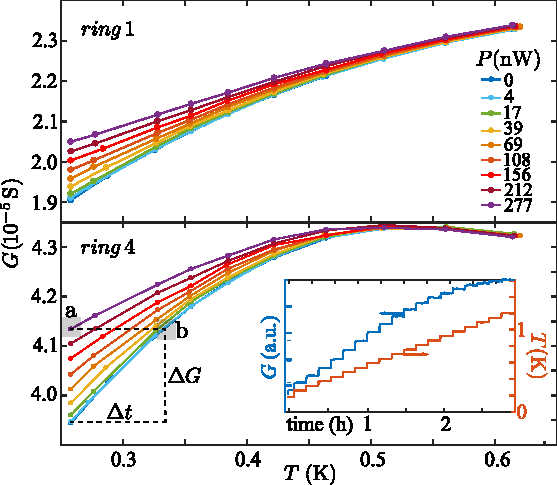
\includegraphics[width=1\textwidth]{figures/temperature_corbino/fig5_calT.pdf}
    \caption{Temperature calibration curves for the innermost (ring 1) and outermost (ring 4) rings. For each temperature and power set, like in Fig. \ref{fig:DCvoltTempCounter}, a point of this plots is obtained. Colors represent different dc heater powers. An interpolation $f(T, G, P)$ is made, from which it is possible to determine a $\Delta t (G) = f^{-1}(G,P)$ for temperatures below $T = \SI{550}{\milli\kelvin}$. It is important to note that both rings are measured simultaneously. \textbf{\textit{Inset:}} Conductance and temperature recorded for $P = \SI{0}{\nano\watt}$.}
    \label{fig:calT}
\end{figure}

From this information we can finally produce a calibration curve like the one shown in Fig. \ref{fig:deltaTpower}. Each point corresponds to the averaged value of the measured temperature difference between rings, i.e. an aproximation of the thermal gradient modulus of the system. The uncertainties include the fitting curves and the statistical error of each point. A deeper understanding and better aproximation of the type B \cite{gum2008} uncertainty should be produced in the future. 

\begin{figure}
    \centering
    \includegraphics[width=0.7\textwidth]{figures/temperature_corbino/deltaTpower_COMSOL.pdf}
    \caption{Temperature calibration curve. Here the temperature gradient measured indirectly between the inner (1) and outer (4) rings are presented. The error bars corresponding to the uncertainty including statistical and interpolated curves. The resulting values of the finite elements modeling of the GaAs crystal for a power of $\SI{277}{\nano\watt}$ is included.}
    \label{fig:deltaTpower}
\end{figure}


In the next section we shall discuss the thermopower response of the system, the model produced from it and the resulting estimated $\Delta T$. 
But we can also estimate the temperature profile using literature values of the thermal conductivity $\kappa$. From the work of Chickering et al.\cite{chickering2013} we deduced a $\kappa_(T = \SI{300}{\milli\kelvin}) \sim \SI{10}{\watt\per\kelvin}$. Using the simulation software finite elements to solve the heat-flow equation given this coefficients a temperature difference of $\SI{2.5}{\milli\kelvin}$ was found between the center and edge of our sample. This results are shown in Fig. \ref{fig:finite elementsDryWet}, there simulations for a wet cryostat (a) and a dry one (b) are shown. The gray area corresponds to the central hole of the Corbino, the ring dimensions are also sketched. Note the deeper slope of the wet system, here the Helium allows a much higher temperature. For further information on this please refer to Appendix \ref{appendixd}. 

\begin{figure}
    \centering
    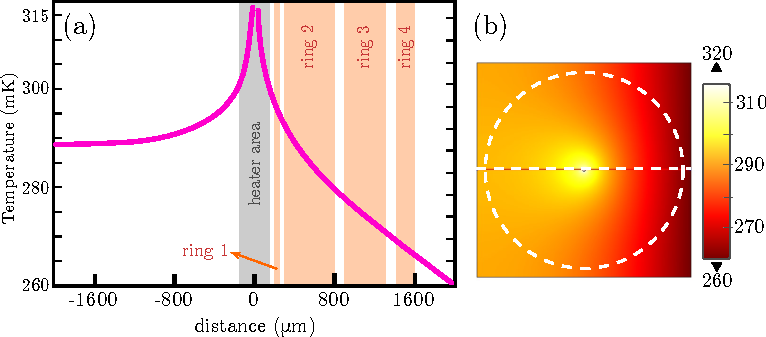
\includegraphics[width=0.7\textwidth]{figures/temperature_corbino/comsol_helium.pdf}
    \caption{Caption}
    \label{fig:finiteElementHe}
\end{figure}

This would lead to a temperature difference across ring 2 of about \SI{1}{\milli\kelvin} that we shall demonstrate to be in good agreement with the value of the thermovoltage theory fit to be discussed. 

\textcolor{violet}{TODO LO ANTERIOR, REVISAR LOS VALORES. TAMBIEN SI LOGRO SACAR BUENOS PLOTS DEL finite elements, INCLUIRLOS ACA Y SEGURAMENTE SERA NECESARIO HACER OTRA SECCION CON ESTO QUE SEA: Heat-flow equation simulation and resulting $\Delta T$}

\begin{figure}
    \centering
    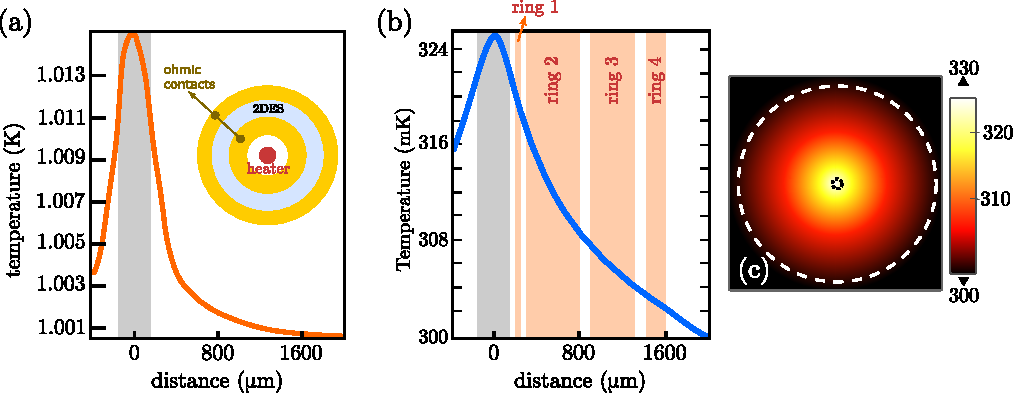
\includegraphics[width=0.9\textwidth]{figures/temperature_corbino/comsol_helium_dry_and_wet.pdf}
    \caption{Temperature profile expected on the samples, produced by a finite elements simulation, original idea by Dr. Werner Dietsche. A central point heating power of P = \SI{277}{\nano\watt} and a standard GaAs thermal conductivity $\kappa = \SI{55}{\watt\per\meter\per\kelvin}$\cite{gaasMTPrus, carlson1965thermal} was used. Sub-figure (a) corresponds to a wet system, while (b) and (c) to a dry one. Notice the faster temperature drop in the case of the wet system. The gray areas indicate sections outside the mesa, where the heater is, wile orange ones to the different Corbino rings. }
    \label{fig:finite elementsDryWet}
\end{figure}


\textcolor{red}{ESTO A OTRO LADO: A note on uncertainty, it must be mentioned that we have not calibrated the LIA under use in this work, they do have a calibration posterior to delivery. They did been verified only against available references.}

\textcolor{red}{OJO CON EL PARRAFO SOBRE EL CERO APLICADO A LA TENSION, ASEGURARSE QUE NO ESTOY MENCIONANDO LA MEDICION DE CALIBRACION DE TEMPERATURA, AHI USABA EFECTIVAMENTE CERO Y UN SMU, SOLO VALE CUANDO HAGO VTP CON EL LOCK IN Y CUANDO HACEMOS CALIBRACION DE TEMPERATURA USANDO }
$f_{\mathrm{in}}= \SI{113}{\hertz}$ unless stated. 





\textcolor{blue}{It is important to note that in our approach the resulting effects and measurements is an average of every direction of the sample, any possible in-homogeneity would be integrated during measurements. But we did not find any signature of such possible effects, like phonon focusing for example.}


\section{sec: Thermovoltage and conductance measurements and modeling}
\label{sec:vtp_g_model}

\chapter{Thermovoltage, conductance and\\ behavior modeling}
\label{ch:vtp_g_model}


We now turn to the thermopower (thermovoltage) measurements and its modeling. As we have already discussed Kobayakawa, et al. \cite{kobayakawa2013diffusion} work presented results for even filling factors and low mobility samples measured at quite high frequencies. Our approach is much conservative. As shown in figure \ref{fig:setupVtpG}.

\begin{figure}
    \centering
    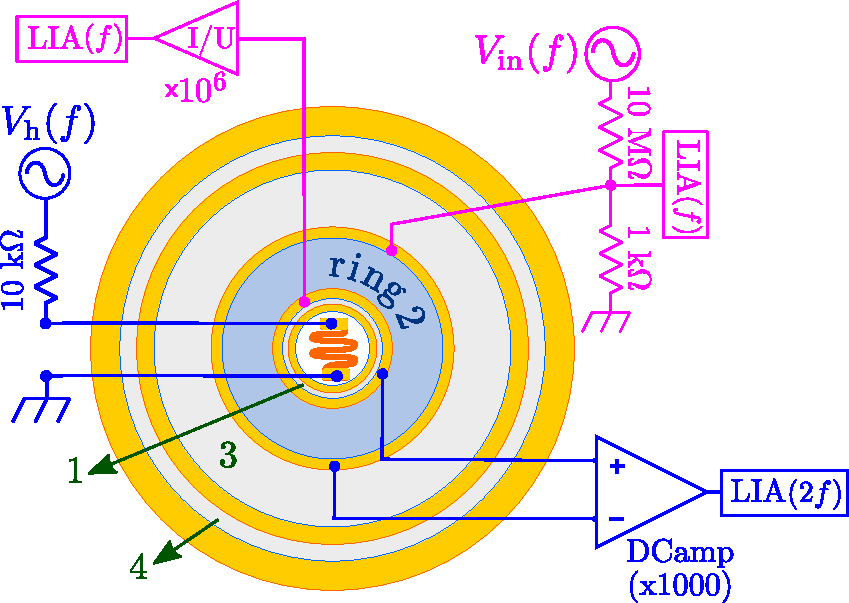
\includegraphics[width = 0.7\textwidth]{figures/vtpGmodel/setup_vtp_g.pdf}
    \caption{Experimental arrangement for the termovoltage (blue) and conductance (pink) measurements. Labels of rings are indicated. The radius of the outermost Corbino is \SI{1650}{\micro\meter}}
    \label{fig:setupVtpG}
\end{figure}

We heat the system by means of the resistive central heater, resulting in a thermovoltage at each Corbino ring. Each of them act independently, 

In order to produce the thermovoltage measurements different configurations were tested. The main problem here being the QH state its conductivity will be competing to the one of the measurement system. To make a proper measurement we must ensure a negligible current, i.e. a measurement system as ideal as possible having the highest possible input impedance. During initial measurements at INTI this became 



Here we will discuss and develop the model we obtained to describe the system and its different behaiviours. In the rest of this discussion it is important to keep in mind the two very different behaiviours of the system:
\begin{enumerate}
    \item Semi-filled Landau Levels (LL), magnetic field around half fractional filling factors $ \nu $ will present metal-like behaivour.
    \item Mobility gap, magnetic fields around integral fillig factors.
\end{enumerate}

We shall discuse them with kind of different aproaches. And we will also consider two dinsctinct behaiviours between low and high magnetic fields. A best definition is given afterwards, but they will be bassically distiguish by the field at which spin splitting in the conductance measurements are found,  in this particular samples $B \approx 1$.

\textcolor{red}{en la parte de caclulo de incerteza del modelo (determinación de $\Delta T$ meter cita a \cite{gum2008, gumModels}}.

\begin{figure}
    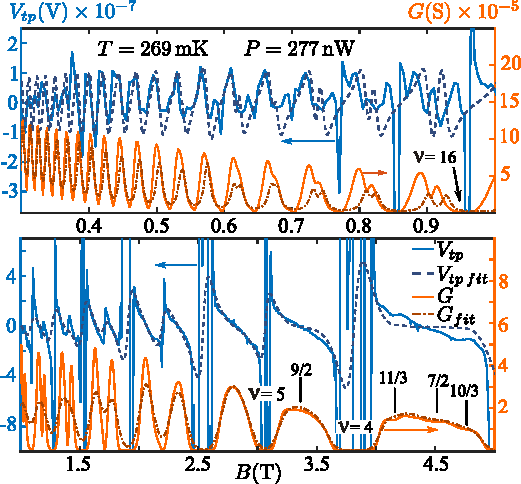
\includegraphics[width = 0.7\textwidth]{figures/vtpGmodel/termovoltageConductance/fig2.pdf}
    \caption{Conductance $G$ and thermovoltage $V_{tp}$ as a function of the magnetic field $B$ for \textit{ring 2} in Fig.~\ref{fig:corbino_exp_setup} at temperature $T$ with power $P$ supplied at the heater.
    Experimental data is plotted in solid lines. Theoretical (dashed) plots  are based on the calculation of 
    \textcolor{red}{eq.~(\ref{onsa})} 
    with the inferred transmission function as explained in (i) and (ii) for the upper and lower panel, respectively.  }
    \label{fig:lowHifield}
\end{figure}


\begin{figure}
    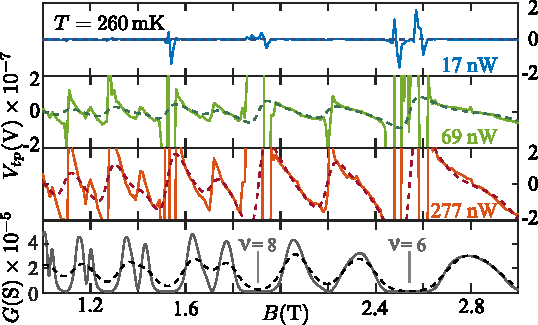
\includegraphics[width=0.7\textwidth]{figures/vtpGmodel/termovoltageConductance/fig3.pdf}
    \caption{Thermovoltage $V_{tp}$  for a fixed temperature and different powers $P^{\prime}$
    applied at the heater, assuming $\Delta T (P^{\prime}) = P^{\prime}/P \, \SI{1.08}{\milli\kelvin}$.
    $P$ and other details are the same as in  Fig.~\ref{fig:lowHifield}.}
    \label{fig:modelHeaterPower}
\end{figure}




\section{Thermoelectric performance}

\begin{figure}
    \centering
    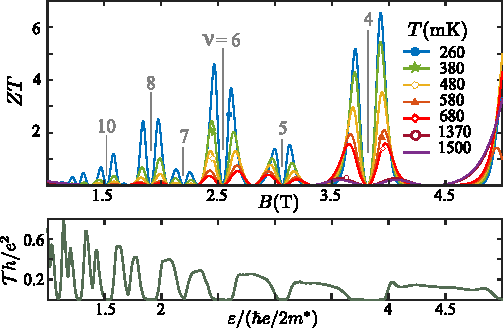
\includegraphics[width=0.7\textwidth]{figures/vtpGmodel/termovoltageConductance/fig5.pdf}
    \caption{Bottom: Transmission function ${\cal T}(\varepsilon)$. Top: Electron contribution to the figure of merit $ZT$.}
    \label{fig:ZT}
\end{figure}
The quality of the thermoelectric performance is evaluated in terms of
the efficiency (for the heat engine), 
 or coefficient of performance (for the refrigerator), which can be parameterized by the figure of merit \cite{benenti2016thermal,benenti2017fundamental}, $ZT = {\cal L}_{21}^2/\mbox{Det}{\hat{\cal L}}$,
 such that the optimal Carnot efficiency/coefficient of performance is achieved for $ZT \rightarrow \infty$.
 %, while $ZT \sim 3$ implies $\eta^{\rm he/fr} \sim \eta^{\rm he/fr}_C/3$. 
 The highest reported values in real materials are between 
 $1 \leq ZT\leq 2.7$ \cite{benenti2017fundamental} while optimistic predictions in the ballistic regime are
 $ZT \sim 4$ \cite{ozaeta2014predicted} or lower.
 In Fig.~\ref{fig:ZT} we show the transmission function ${\cal T}(\varepsilon)$ used to fit the experimental data of Fig.~\ref{fig:lowHifield} within the high-magnetic field regime. We see that the sequence of sharp features at the LL realize energy filters, leading to large values of  $ZT \sim 6$. 
We stress that this analysis is based on the assumption that the main contribution to the thermoelectric and thermal transport is due to the electrons.
Purely phononic thermal transport could tend to decrease the performance.






\textcolor{red}{METER lo de abajo en el texto anterior}

In the presence of disorder and absence of electron-electron interactions ${\mathcal T}(\varepsilon)$ was originally calculated by Jonson and Girvin \cite{jonson1984thermoelectric}. At high temperatures, electron-phonon interaction gives rise to an additional component to the transport coefficients ${\cal L}_{ij}$. The corresponding thermopower has been studied  in bar geometries for specific filling factors \cite{tieke1996even,zhang2004oscillatory} and, more recently, in illuminated Corbino samples \cite{Zalinge2003}, while no signatures of electron-phonon interaction were found in other experimental works in the Corbino geometry \cite{kobayakawa2013diffusion}.
The thermal conductance has an additional component of purely phononic origin. We have only very limited access to this transport coefficient with the present experimental setup.

\chapter{Quality and Innovation}
\label{ch:qi}


\textcolor{red}{Esto puede ir probablemente como apéndice, aunque desde el punto de vista político convendría dejarlo como capítulo, tengo que reveer cómo juntar en uno calidad e innovación simultáneamente. Lo tuve que resumir muchísimo para que no sea una pesadez de lleer. Otra opción sería meter conclusiones principales desde el punto de vista innov y quality management in processes, eg. outputs check within the quality system of the institution and colaborators, periodic revision of objectives and results, etc. And then just mention that innovation and quality management were taken into account, and refere the reader to a web page containing the works produced during the thesis (in spanish, the ones I already have.). This would reduce significantly this section but would show that we took into account what we learn during the different courses. TO DISCUSS WITH ALE}

From the point of view of quality and innovation this thesis must be thought from the main outputs to the laboratory, which will be the main receipt of its developments. It is important to remember that expenditures on R \& D are a capital formation activity, i.e. investment 
\cite[Foreword]{frascati}. And in today\'s world this is one of the formost pillars in the development of countries and technology economies. It is my strong believe that the development of cutting edge technologies should be one of the goals of our society, and should result in an improvement of the lives of our countryman. 

We include the quality and innovation (Q \& I)) studie at the end, mostly because it is not easy to discuss it without the context of the research and development (R \& D) already explained. And becomes clearer if we do not have to explain the develpments and the Q \& I simultaneously. Nedless to state, that the following was taken into account on the initial steps of the R \& D process, and updated during the course of this thesis.

The initial objective of the thesis was quite large, \textit{to study and develop methods to determine, measure and apply thermoelectric properties of quantum Hall states with application to metrology. } As we have dicussed during the text, we focused on Corbino devices resulting in 
\begin{enumerate}\label{enum:developments}
    \item Gradient temperature determination by measuring and modeling the system.
    \item Thermopower measurements.
    \item Thermopower modeling.
    \item Thermal current modeling.
\end{enumerate}

The gradient temperature determination presented provides a way to determine such gradient by means of a calibrated sensor in a different section of the system, but relies on it. Also, this was proven to work in a cold-finger system, its use in a wet system could be problematic (see \ref{ch:exp} \textcolor{red}{tal vez citar párrafo específico}).

From the point of view of determine absolute temperatures on the system, there is also cavits. The method described in \ref{ch:temperature_corbino} can be applied to obtain a \textbf{relative} temperature change of the system (2DES). It is not possible from it to provide an absolute value of temperature. But, importantly, such change it is very important too, since the calibrated sensor is not determing the actual temperature of the 2DES (system to measure), not even the crystal temperature containing it. It provides then, a mean to measure temperature changes during measurements. 

The thermopower measurements provided two main outputs: the development of high resolution measurements and unexpected behaivour of the 2DES under the QH \textcolor{red}{incluir QH en glossary} state. 

The thermopower modeling resulted in a model \ref{ch:vtp_g_model} that describes the system in the semi-filled LL and returns a value for the temperature gradient obtained 
\footnote{This gradients corresponds to the AC responses. In the model \ref{ch:vtp_g_model} and experimental \ref{ch:vtp_g_model} sections further explanation of this important detail are given.}.
As we have discussed the measured thermopower in and out of phase was not expected, not even its maximum values. We were able to produce a model that at least provides an explanation of these behaviors, based on the measurements.

Finally the semi-filled LL model was further developed to predict the thermal currents of the systems. From the model point of view, it predicts a very interesting behiviour, that could be exploited to cool down sections of a system. This yet remains to be experimentally proven.

All itemized cases fulfill the cryteria to be considered an R \& D activity. They have benn proven to be \textit{novel}, since all of them have been peer reviewd and published, \textit{creative} the results and models produced are not obvious and resulted in possible new applications (cooling). As most cutting edge studies they result to be \textit{uncertain}, we new we were able to produce devices and measurements, but by no means we were expecting several outcomes that we have described. As always in science, and specially in metrology we have produced very \textit{systematic} studies, that are also \textit{reproducible} between laboratories (Argentine and Switzerland) and devices. So the basis of our studies comply with all requirements of R \& D.

Stablished this, we can analize the threats and opportunities of the project (context). By using a innovation management tool and taking into account any thinkable possible theat and opportunitie both internal or external (macro and micro), we produced a scheme resuming such posibilities \ref{fig:innov-theats_opportinities}. This figure also includes some possible scenarios, that resulted to be out-of context. 

\begin{figure}
    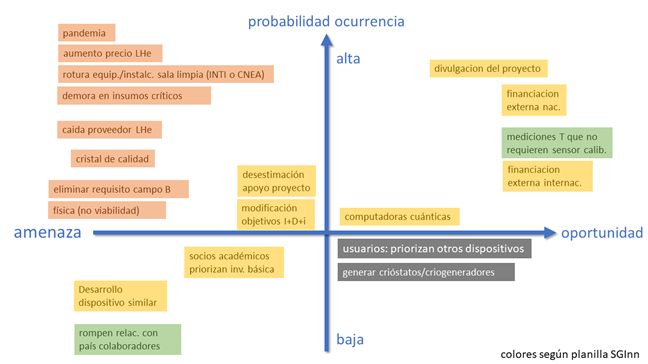
\includegraphics[width=0.9\textwidth]{figures/innovation/theatsOpportunitiesInnov.png}
    \caption{Opportunities and threats of the project, they are plotted against its degree of occurrence probability. Their resulting score is given by color, being redish a high-priority, yellow mid-priority and green low-priority theats. Meanwile high priority opportunities are green, yellow mid priority and finally grey resulted in out of context opportinities.}
    \label{fig:innov-theats_opportinities}
\end{figure}

For each one of this possible factors a possible solution-alternative and course of action was evaluated. We will not indicate each one of them, but for example, it is usual that the micro-machining facilities find working problems that could result in heavy delays in our goals. To overcome such possibilities we had the chance to work in two near facilities (INTI and CNEA). This was a very interesting situation, since it resulted in a nice flexibility at the time to produce our devices.

\section{Interested Parties}
\label{sec:interested_parties}

As in context, the interested parties were studied by Q \& I tools. One important point is that this project was self generated, and that the temperature determination of the systems is to be use in the Quantum Standards Laboratory. But, any possible development in this regard could be implemented in other institutes working on cryogenic measurements under magnetic fields. There are superior tecnologies, but its implementation and development (most not comercial) would require long development times, cyostat modifications and clean room facilities not easely accesible, e.g. Johnson noise thermometry \cite{Johnson1928,nyquist1928,qu2019johnson} that would imply the development from scratch of such tecnology in our laboratory 
\footnote{This being said, is my firm believe that our institute should start steps forward this technology in the comming years, it is becoming a standard \cite{flowers2017boltzmann,Department2013}.}.

Commercial resistive and semiconducting sensors are available for cyogenic systems, most of them are quite large, very expensive (particularly the calibrated ones) and they do not provide the 2DES temperature, they measure usually some part of our cyosystem. Any group working with high fields and low temperatures could become interested in any tecnology providing the kind of measurment developed in this thesis.

The interested parties are detailed in \ref{fig:innov-interested-parties}, from the analisys tools we obtain that the local and external research groups present no applicable action, the same happens regarding cryogenic companies. En both cases the influece power is big but the interest at this time is low, the only way to improve this is to obtain a working prototype to develop specific actions.
Since the development is to be applied in a national institution, the Nation is represented as an Argentine map, which supports the development and the institutions undertaing it. It is a group which influence power is high but its interest for now very low.  Because of this its participation should be kept and must be informed in the best way possible. There are only scarse cases wne this group increses its interest, a good positive example are the innovations and research regarding COVID19, satellites (in is final lounch stage), and such. 

Of course our collaborators (national and international) are one of the main influece parties, resulting to be in the direct interest group, in the same way as the national institutions involved, like INTI, UNSAM and the parties directly involved in the develpment of this thesis.
The case of INCALIN-UNSAM is double, since its aim is to increse local develpments and to show how research, quality and innovation can be applied to local cutting edge technologies.

\begin{figure}
    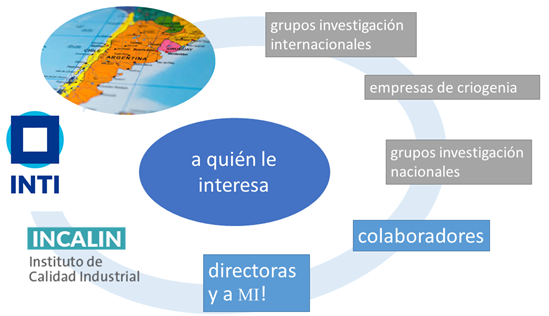
\includegraphics[width=0.8\textwidth]{figures/innovation/interested-parties.png}
    \caption{Small schematic figure indicating the evaluated possible interested parties by means of the quality and innovation tools used.}
    \label{fig:innov-interested-parties}
\end{figure}

Given all what we have discussed, and the usual technology readiness level scales, see Fig.~{fig:innov-trl}, we can set scales for the developments itemized initially~\ref{enum:developments}
\begin{figure}
    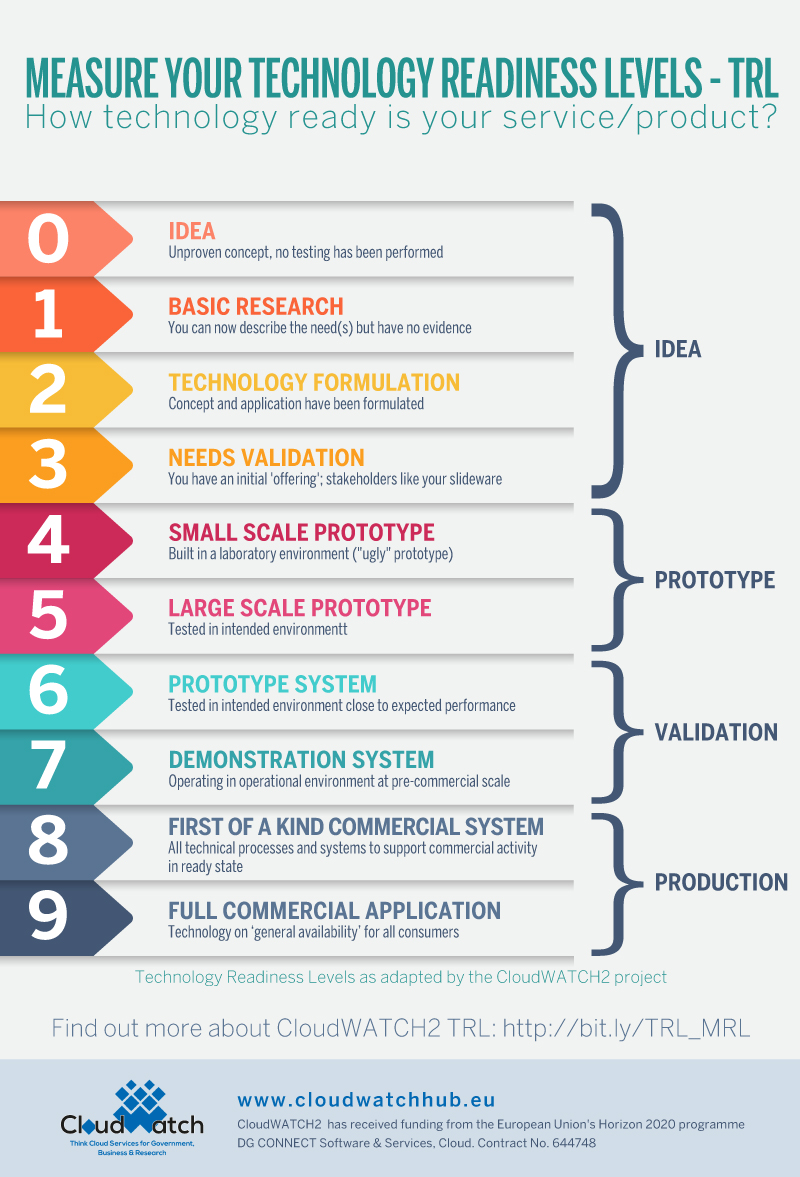
\includegraphics[width=0.8\textwidth]{figures/innovation/trl.jpg}
    \caption{\textcolor{red}{tengo que hacer el propio}}
    \label{fig:innov-trl}
\end{figure}


\textcolor{red}{citar: \cite{frascati,osloManual,pmbok2021guide}}

\textcolor{red}{Incluir acá o en la sección inicial \url{https://www.bipm.org/documents/20126/43742162/CIPM-MRA-G-13.pdf/f8b8c429-42e0-4cf1-dc6c-bc60ab7f371a} y \url{https://www.bipm.org/documents/20126/43742162/CIPM-MRA-P-11.pdf/} Donde se explica el MRA, esto es hyper relevante respecto a cómo impactamos. Desde el punto de vista del MRA, toda mejora va relacionada directamente a las CMCs declaradas de Argentina. De esto hablé un poco en el trabajo de Calidad enfocada a procesos, no lo incluí acá aún. En esa misma dirección habría que incluir la ISO 17025 }





\chapter{Future work possibilites}
\label{ch:future}

\emph{Future ideas to be implemented, things that we should prove (measure paper). See One Note CSC ideas.}
\chapter{Conclusion}
\label{ch:conclusion}

\emph{A conclusion...}

\textcolor{blue}{INcluir una discusión sobre el Vtp}

The measurements show that there are two outputs, an in-phase resistive (ip) and out-of-phase (op) components. They are not shown in previous works (CHECK THIS!). Initial calculations taking into account an original idea of Dr. Arrachea, taking a capacitive effect into the edge-channels, comming from a redistribution of charge might help to understand them.

Incluir dibujo

Resulting in contributions of the form
\begin{align}
    \vtpout &= \frac{\capac \omega T}{\left(\capac \omega T \right)^2 + \onsa{11}^2} \left(  \onsa{12} - \onsa{11} \Delta T \right)\\
    %
    \vtpin &= \frac{-1}{\left( \capac \omega T \right)^2 + \onsa{11}^2} \left(  \onsa{11} \onsa{12} + \left( \capac \omega T \right)^2 \mathcal{D} \right) \Delta T \\
    %
    \mathcal{D} &= \frac{\mathcal{D}^{\mu}}{\mathcal{D}^{T}}
\end{align}
%
CHECK D DEFINITION AND INCLUDE ITS RELATION TO DENSITIES, ALSO INCLUDE THE DEFINITION OF C, THAT DEPENDS ON SEVERAL OTHER CAPACITANCES.
%\input{mainmatter/chapter} % file to be added


%% Letters for chapters
\appendix

\chapter{Appendix A}
\label{appendixa}

\section{Clean room recepies and laboratory techniques}

\textcolor{red}{incluir los diferentes pdf que fui preparando}

\chapter{Appendix B}
\label{appendixb}

\section{Sample properties}

\textcolor{red}{incluir acá todos los pdf de las muestras usadas. Probablemente necesite el aproval de WD. Charlar si creemos que esto sea crítico o no. Como en el caso de las mediciones, tal vez se puede poner características generales y de ahí decir que son entregados al lector "upon request".}
\chapter{Appendix C}
\label{appendixc}

\section{Extra information in some measurment systems}

\textcolor{red}{Incluir los detalles de algunos instrumentos como el amplificador DC, el crióstato wet y dry, el amplificador que hicimos nosotros y otros sistemas que sean relevantes del texto y no tengan publicado un manual online.}
\chapter{Appendix D}
\label{appendixd}

\section{Extra information on the finite elements simulation} 

To predict an approximate behaivour of the GaAs/AlGaAs system as a heat conducting device some numerical simulations solving the heat-flow equation over different configurations and contour conditions were made.

\textcolor{red}{seria lo ideal realizar las simulacines en 3D incluyendo los contactos metálicos, éstos van a modificar el perfil de temperatura y sumar una corrección al resultado modelado. Esto puede llevar tiempo, sólo incluir si se puede. Lo mismo respecto a un promedio ponderado integrando en una curva en el Corbino, para esto tengo que entender cómo hacer interacturar al Matlab con el comsol y de ahí armar un programa que lo haga. Sólo si se llega.}

The radiation was not taken into account, a small calculation shows that it is negligible over the conduction effect, we just need to write the Stephan-Boltzmann equation. Here we can assume the worst case possible, i.e. emmisivity $ \varepsilon = 1$
\begin{equation}
    P_R(T) = \varepsilon \sigma A T^4 = \sigma (\SI{50}{\micro\meter})^2 (\SI{300}{\milli\kelvin})^4 = \SI{3.6E-9}{\nano\watt}
\end{equation}



%\input{appendix/appendix-AA} % add an appendix from file appendix-AA.tex



%% Add bibliography
%%%%%%%%%%%%%%%%%%%%%%%%%%%%%%%%%%%%%%%%%%
\Urlmuskip=0mu plus 1mu\relax % avoids urls to run into margins in bibliography
\bibliographystyle{IEEEtran} % Bib style IEEEtrans: appearance order and numbered citations
\bibliography{PhDthesis2} % Entries are in the PhDthesis2.bib file. You should check some paper management software and scholar.google.com to produce this file. You can find some relevant info at: https://github.com/realmariano/wiki_labo



\end{document}
%%%%%%%%%%%%%%%%%%%%%%%%%%%%%%%%%%%%%%%%%%%%%%%%%%%%%%%%